%!TEX root = ../../../adrien_gomar_phd.tex

\subsection{Analysis of the convergence}
\label{sub:dream_ls_conv_coeff}

The convergence of the steady computation using the Roe~2 space scheme
is reported in Fig.~\ref{fig:dream_ls_convergence_roe2}. The residual
show a four order of magnitude decrease and the similarity
coefficients are convergence starting at 500~iterations.
Therefore, according to \citet{Casey2000}, the
solution is considered to be converged.
\begin{figure}[htb]
  \centering
  \subfigure[residuals]{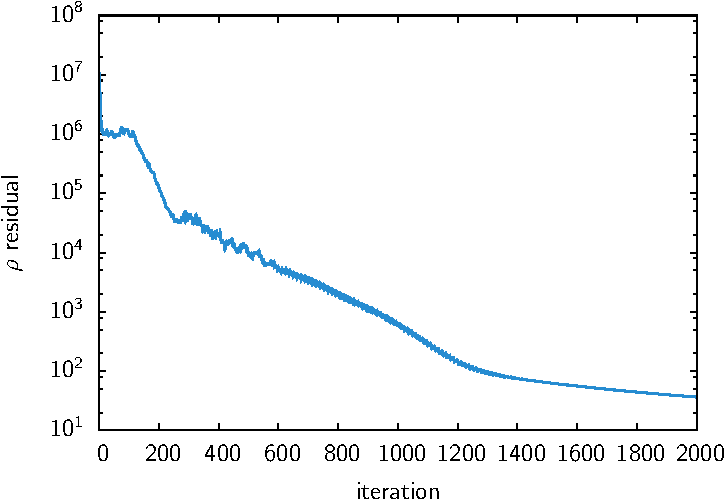
\includegraphics[width=.35\textwidth]{DREAM_LS_RESIDUALS_PPT.pdf}}
  \subfigure[$C_T$]{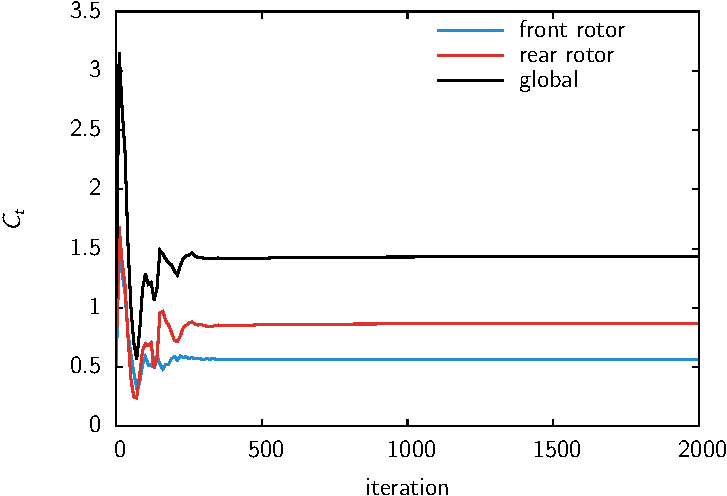
\includegraphics[width=.35\textwidth]{DREAM_LS_FORCES_CT_PPT.pdf}}
  \subfigure[$C_P$]{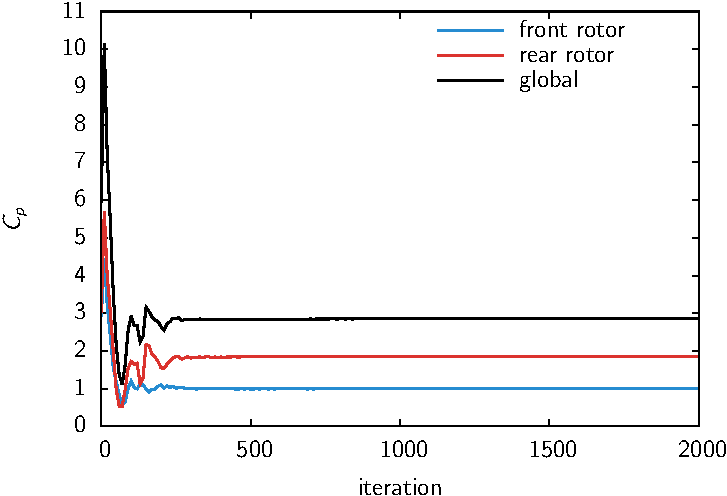
\includegraphics[width=.35\textwidth]{DREAM_LS_FORCES_CP_PPT.pdf}}
  \subfigure[$\eta$]{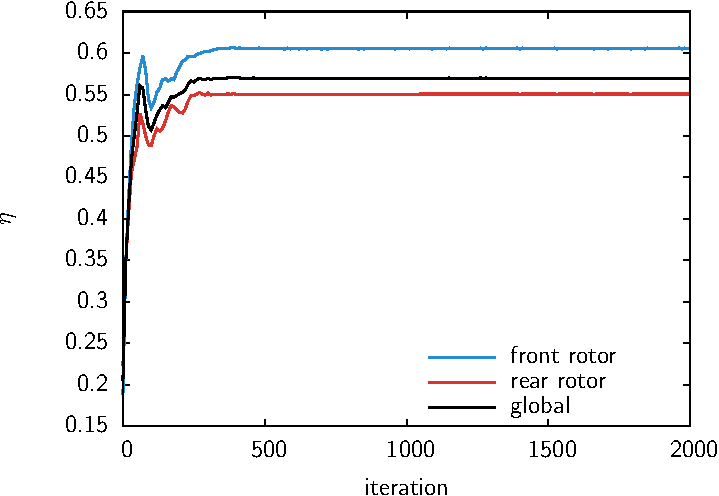
\includegraphics[width=.35\textwidth]{DREAM_LS_FORCES_ETA_PPT.pdf}}
  \caption{Low-speed isolated configuration: convergence of the steady
  computation.}
  \label{fig:dream_ls_convergence_roe2}
\end{figure}

\subsection{Similarity coefficients}
\label{sub:dream_ls_sim_coeff}

The similarity coefficients as defined in 
Sec.~\ref{sub:cror_similarity_coeff} are computed on
this steady results and reported in Tab.~\ref{tab:dream_ls_sim_coeff}
\begin{table}[htb]
  \ra{1.3} \centering
  \begin{tabular}{ccc|cccccc}
    \toprule
    $C_T$ & $C_P$ & $\eta$ & $C_{T_f}$ & $C_{P_f}$ & $\eta_f$ & $C_{T_r}$ & $C_{P_r}$ & $\eta_r$ \\
    \midrule
    1.1319 & 2.0927 & 0.5726 & 0.5637 & 0.9941 &  0.6002 & 0.5682 & 1.0986 &  0.5475 \\
    \bottomrule
  \end{tabular}
  \caption{Low-speed isolated configuration: similarity coefficients.}
  \label{tab:dream_ls_sim_coeff}
\end{table}
The results are consistent with the efficiency estimation given in 
Eq.~\eqref{eq:estimation_sim_coeff} for a take-off propeller.
In fact each rotor of the CROR have an efficiency that is between $0.5$
and $0.8$. The advantage of the CROR is demonstrated as the rear
rotor is able to retrieve a thrust coefficient of $0.5682$ while
the front rotor alone would only give $0.5637$.
The second rotor allows thus to more than double the thrust of the engine.
However, the efficiency is affected compared to an isolated propeller, as
it goes from $0.6002$ for the front rotor to $0.5726$ for the CROR.
Nevertheless, achieving such a level of thrust coefficient on an isolated
propeller would require a higher loading of the blades. This is another advantage 
of the CROR engine, two rotors are used to create the thrust which allow to
reduce the loading of each rotor compare to an isolated propeller and thus
allow higher Mach numbers. In fact, the rotation of the rotors is reduced 
to maintain a subsonic Mach number while not degenerate the efficiency.


\subsection{Radial profiles}
\label{sub:dream_ls_radial_profiles}

Six radial profiles are extracted,
positioned as shown in Fig.~\ref{fig:dream_ls_position_radial}
using Antares (see Appendix~\ref{app:antares}). The absolute
Mach number, absolute flow angle, static pressure, static
temperature, stagnation pressure and stagnation temperature
are shown in Fig.~\ref{fig:dream_ls_radial_profiles}
against the radial position expressed
relative to the radius of the front rotor blade.

The absolute Mach number, show in 
Fig.~\ref{fig:dream_ls_radial_profiles_ma}, is constantly increased through
the two rotors as it goes from the inflow condition value $M=0.2$
up to $M=0.4$. Note that above $R/h=1$, the Mach number
almost recovers the inflow condition. Moreover, it can be infer from the
$M_a$ evolution, that the stream tube is contracting.

The motivation for adding a second rotor to a propeller
was to recover the energy lost by the swirling flow
(recall Sec.~\ref{sub:cror_velocity_triangle}).
The absolute angle of the flow is shown in 
Fig.~\ref{fig:dream_ls_radial_profiles_alpha}. The front rotor
deviates the absolute velocity of almost $20^\circ$, justifying the need
for a second rotor. Between the fourth and the fifth extraction plane, namely
passing through the rear rotor, straighten the flow up. In fact,
the deflection angle is now close to $0^\circ$ for $0.3 \leq R/h \leq 0.7$.
Below that, the deflection angle remains negative. In the tip vortex region
of the rear rotor, one can the effect of the two tip vortices: between 
$0.8 \leq R/h \leq 0.9$, the front rotor tip vortex is seen as the 
deflection angle is positive, which is consistent with the positive
peak observe near the blade tip region in plane $P3$ and $P4$.

The goal of a CROR is to create thrust through an acceleration of 
the flow, not to produce static pressure as in a compressor stage.
This is highlighted in Fig.~\ref{fig:dream_ls_radial_profiles_ps}
where the evolution of the static pressure is shown.
In fact, the evolution of the static pressure lies with 2~\%
of its inflow value. A small increase is observed at each
rotor crossing. Upstream the rotors, the potential effects can
be seen. Actually, the flow is accelerated by the rotors, this acceleration
yielding a decrease of the static pressure 
(roughly through the Bernouilli theorem) and this pressure deficit is observed in
planes $P1$, $P2$ and $P4$.

The stagnation pressure evolution is shown in 
Fig.~\ref{fig:dream_ls_radial_profiles_pi}. As the static pressure
and the absolute Mach number is grows along with the crossing of the rotors,
it is logical to have an increase in the stagnation pressure.
It is actually a marker of the energy exchanged between the rotor
and the fluid.

Figure~\ref{fig:dream_ls_radial_profiles_ti}
shows the stagnation temperature.
An increase is observed at each 
rotor crossing. This is consistent with the
Euler theorem that states that the variation of total enthalpy (roughly
the stagnation temperature) is equal to the variation of the product of
the azimuthal deflection of the fluid and the rotation velocity. As a rotor
deviates the fluid, the stagnation temperature should increase, 
hence the consistence.
\begin{figure}[htb]
  \centering
  \subfigure[position of the extraction planes]{
    \label{fig:dream_ls_position_radial}
    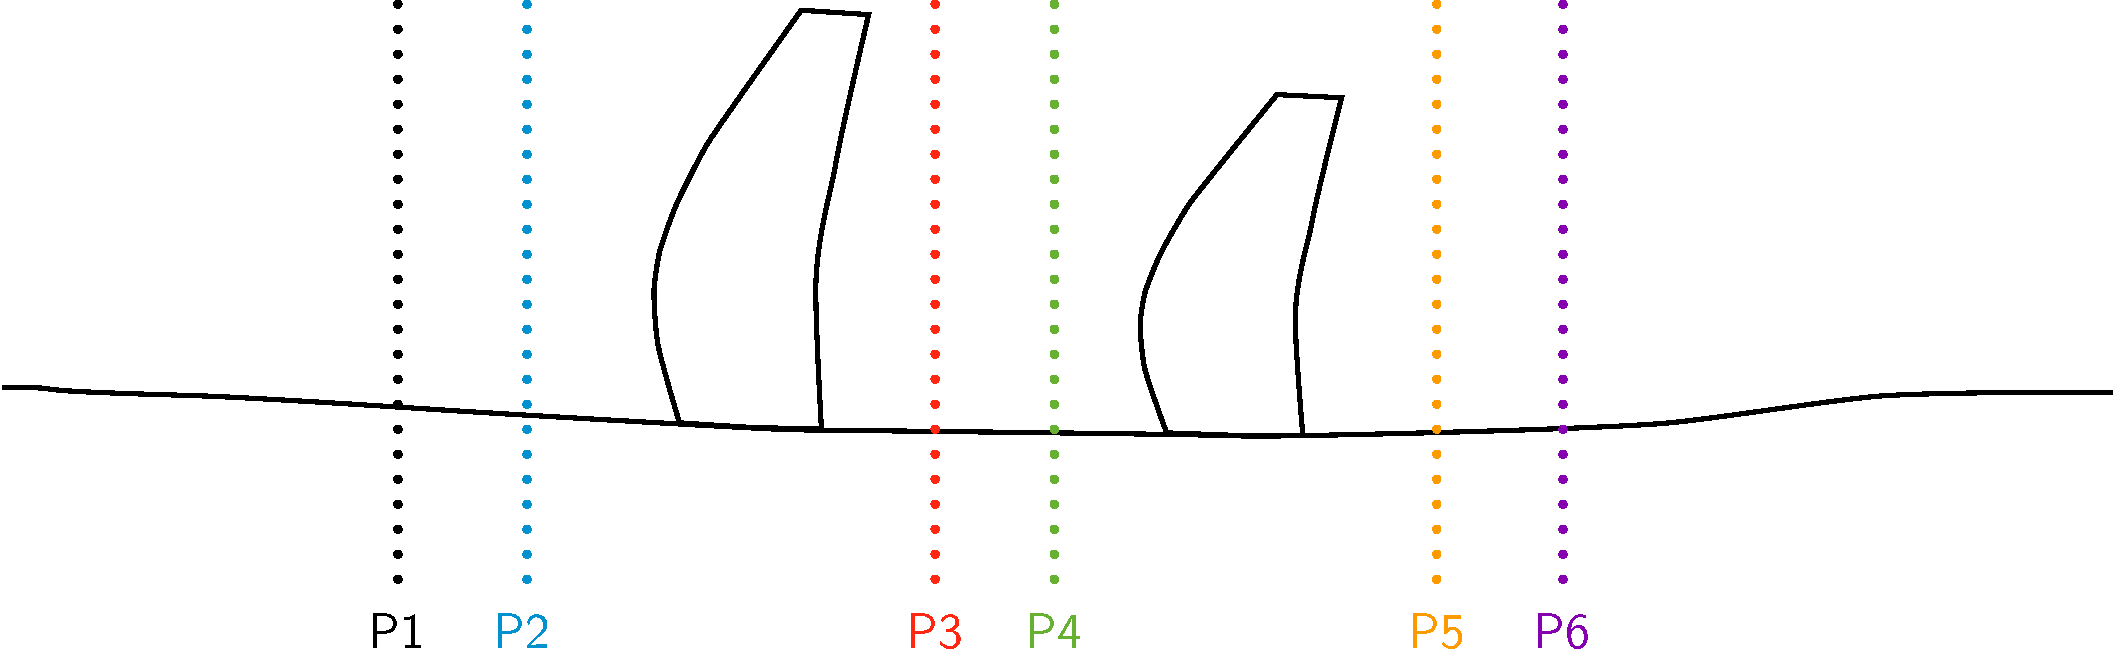
\includegraphics[width=.55\textwidth]{dream_position_azi_mean.pdf}}
  \subfigure[absolute Mach number]{
    \label{fig:dream_ls_radial_profiles_ma}
    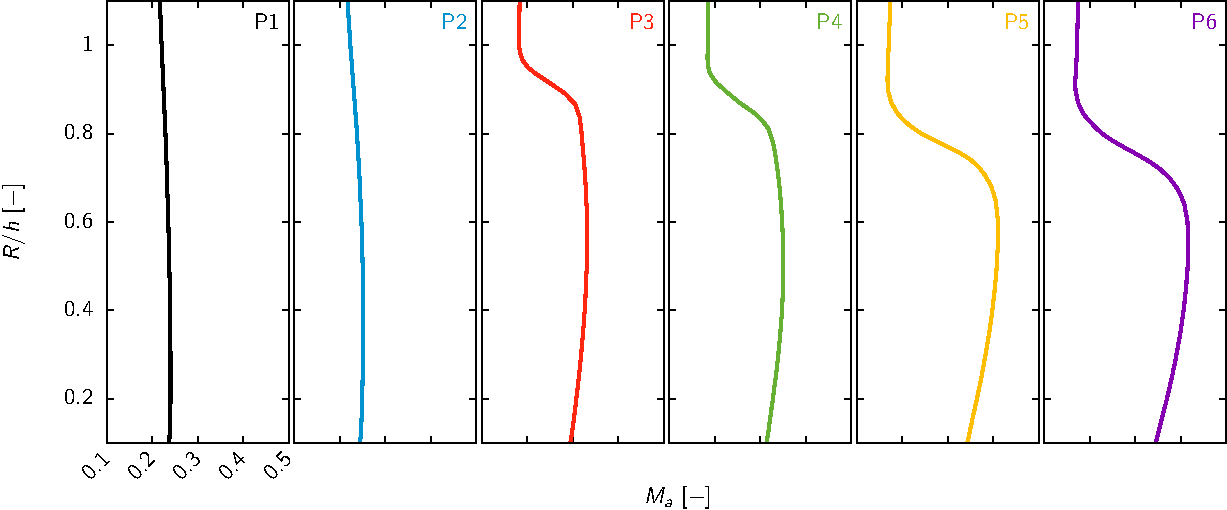
\includegraphics[width=.72\textwidth]{DREAM_LS_RANS_AZI_MEAN_PPT_macha.pdf}}
  \subfigure[absolution flow angle]{
    \label{fig:dream_ls_radial_profiles_alpha}
    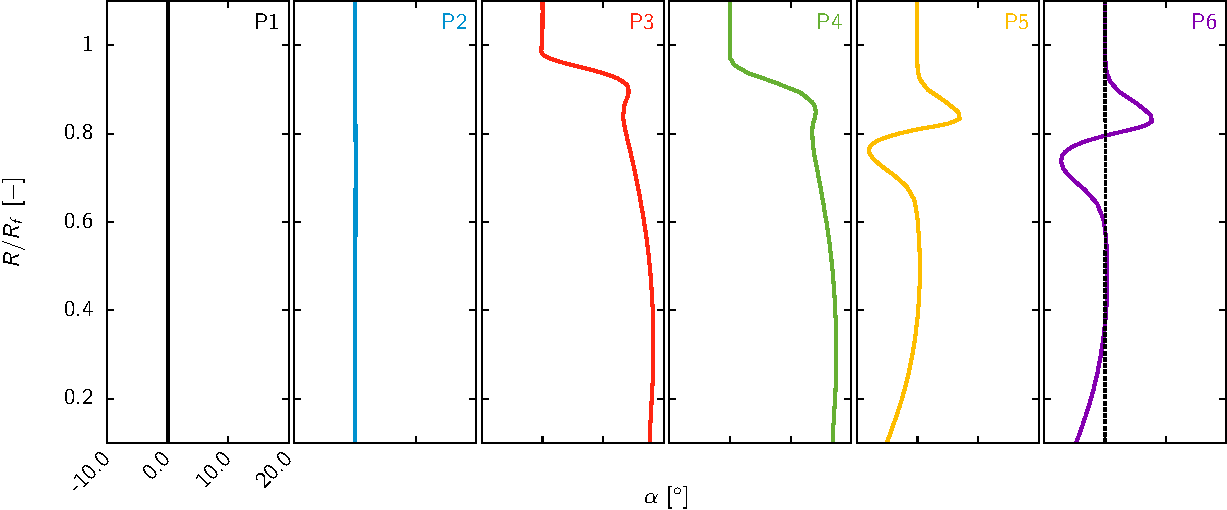
\includegraphics[width=.72\textwidth]{DREAM_LS_RANS_AZI_MEAN_PPT_alpha.pdf}}
  \caption{Low-speed isolated configuration: radial profiles.}
\end{figure}
\setcounter{figure}{\value{figure}-1}
\begin{figure}[htb]
  \centering
  \setcounter{subfigure}{3}
  \subfigure[static pressure]{
    \label{fig:dream_ls_radial_profiles_ps}
    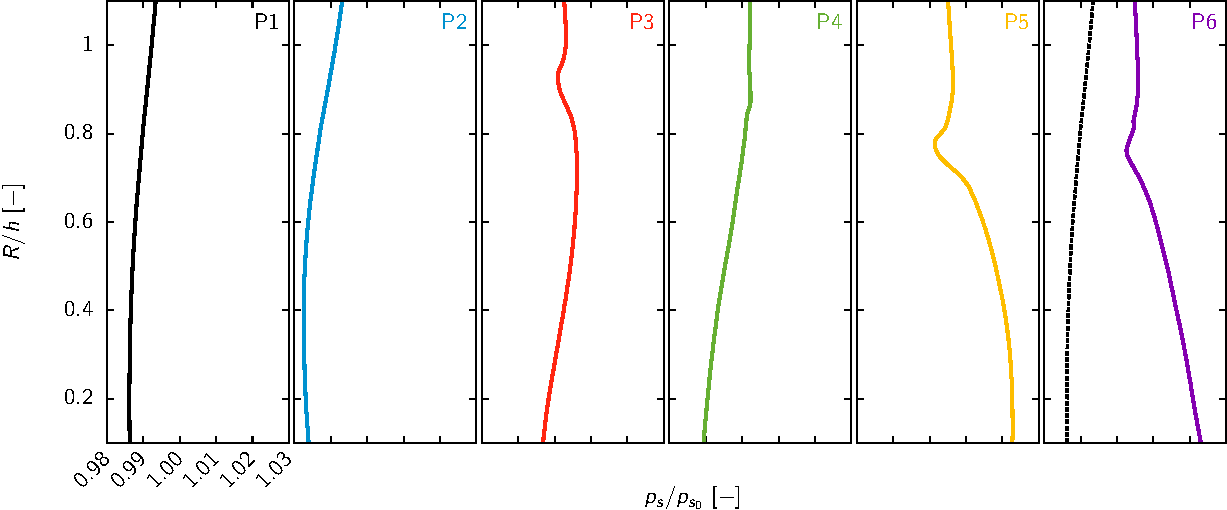
\includegraphics[width=.72\textwidth]{DREAM_LS_RANS_AZI_MEAN_PPT_ps.pdf}}
  \subfigure[stagnation pressure]{
    \label{fig:dream_ls_radial_profiles_pi}
    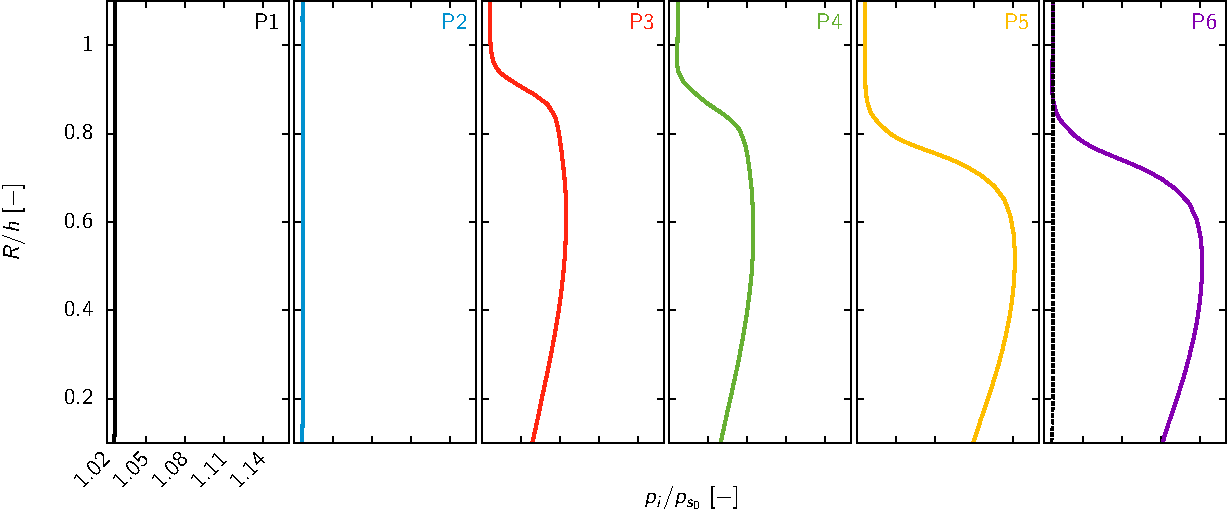
\includegraphics[width=.72\textwidth]{DREAM_LS_RANS_AZI_MEAN_PPT_pi.pdf}}
  \subfigure[stagnation temperature]{
    \label{fig:dream_ls_radial_profiles_ti}
    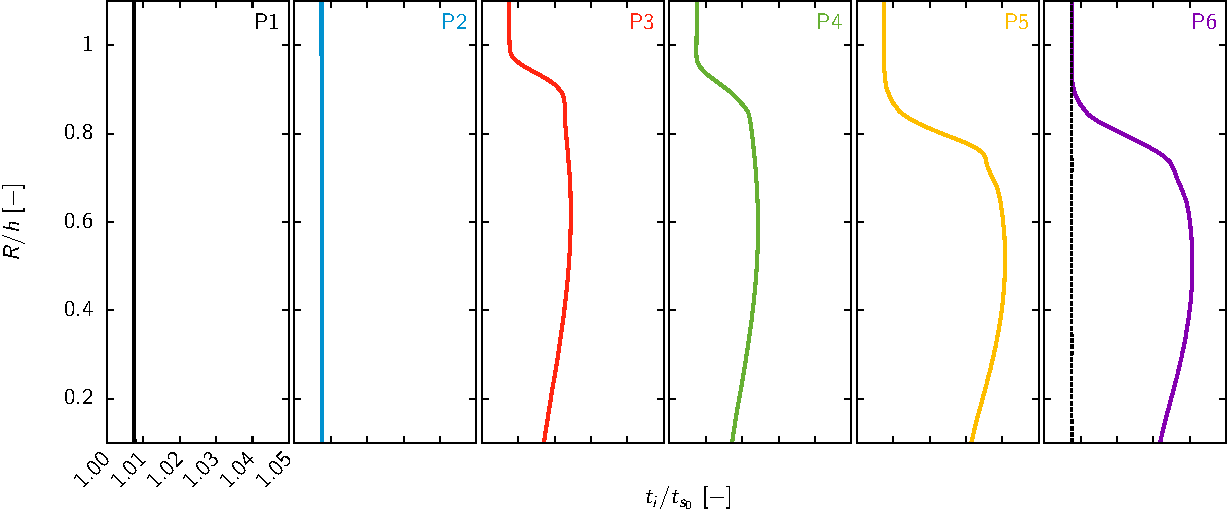
\includegraphics[width=.72\textwidth]{DREAM_LS_RANS_AZI_MEAN_PPT_ti.pdf}}
  \caption{Low-speed isolated configuration: radial profiles (contd.).}
  \label{fig:dream_ls_radial_profiles}
\end{figure}

These 1D results provide us confidence. In fact, the flow physic that
was expected is observed in the results. To further analyze the simulation,
2D results are presented in the following section.

\subsection{Flow field around the blades}
\label{sub:dream_ls_flow_field}

Contours of the relative Mach number are shown in 
Fig.~\ref{fig:dream_ls_mach_kp} along with the pressure coefficient
for both the front and the rear rotor
$k_p$ defined as:
\begin{equation}
   -k_p = - \frac{p_s - p_{s_0}}{\rho n^2 D^2},
\end{equation}
where the $n$ and $D$ parameters are the one of the front rotor
to ease the comparison.

The $- k_p$ should be interpreted as follow, an increasing $- k_p$
means that the pressure gradient is negative, namely the flow
is accelerating. Therefore, the positive  $-k_p$ range is attributed
to the suction side and the negative to the pressure side.
The stagnation point is highlighted
by the minimum of the pressure coefficient. On the pressure side 
($-k_p < 0$) the flow then accelerates
toward the trailing edge with a favorable pressure gradient. 
On the suction side, a rapid acceleration of the fluid
is observed near the leading edge 
($\partial (-k_p) / \partial x \gg 0$) followed by
a deceleration of the fluid along with an
adverse pressure gradient.
Nevertheless, the velocity of the fluid is always superior
on the suction side compared to the pressure side.
On the front rotor, the integrated pressure coefficient is
increasing with the increase of the relative span, at least 
when comparing the 50~\% and the 75~\% relative spans.
After that, the pressure coefficient is almost constant on 
the front rotor. The loading is thus almost constant for
relative spans greater than 50~\%. In the propeller community and
by extension the CROR community~\cite{Bousquet2012}, the loading of a blade is known
to be maximal for a relative span of 75~\%, which is consistent
with our results.
The pressure coefficients on the rear rotor have a similar shape
than the one of the front rotor. However, the loading is
larger on the rear rotor and near the tip of the blade
$R/h > 75~\%$, the integrated value of the pressure coefficient
increases drastically. This is highlighted by the thrust coefficient 
of the rear rotor $C_{T_f}$ which is reported in 
Tab.~\ref{tab:dream_ls_sim_coeff} and that is higher than
the front rotor coefficient, even though the diameter of the front
rotor is chosen to adimensionnalize the pressure coefficient which
lessened the loading of the rear rotor.

The relative Mach number contours are also shown in 
Fig.~\ref{fig:dream_ls_mach_kp}.
As inferred by the tip Mach number value $M_{tip}$ of the blade
given in Tab.~\ref{tab:dream_ls_flight_condition},
the relative Mach number does not 
cross the supersonic boundary $M_{rel} = 1$.
The flow remains thus subsonic which is, aerodynamically speaking,
a good feature for the performances since shocks create losses.


\begin{figure}[htb]
 \centering
 \begin{tabular}{rccc}
   & $-k_p$ front rotor
   & $-k_p$ rear rotor
   & relative Mach number\\
   \rotatebox{90}{\qquad\qquad 25~\%} 
   & 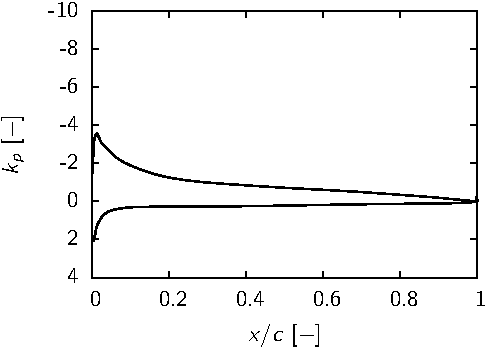
\includegraphics[width=0.28\textwidth]{DREAM_LS_KP_25_FRONT_PPT.pdf}
   & 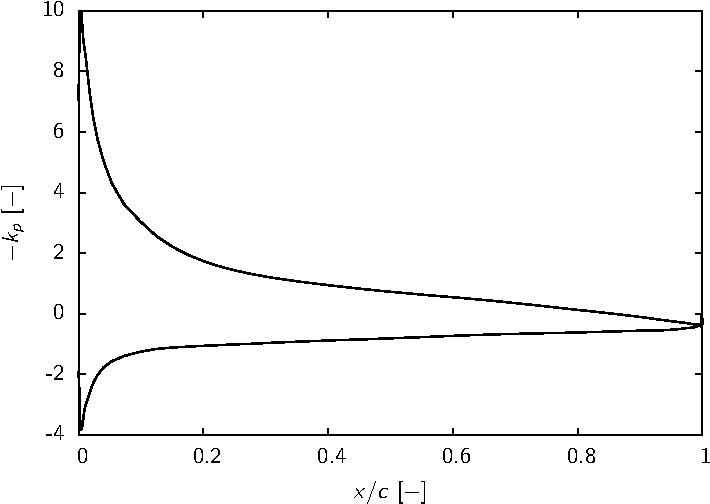
\includegraphics[width=0.28\textwidth]{DREAM_LS_KP_25_REAR_PPT.pdf}
   & 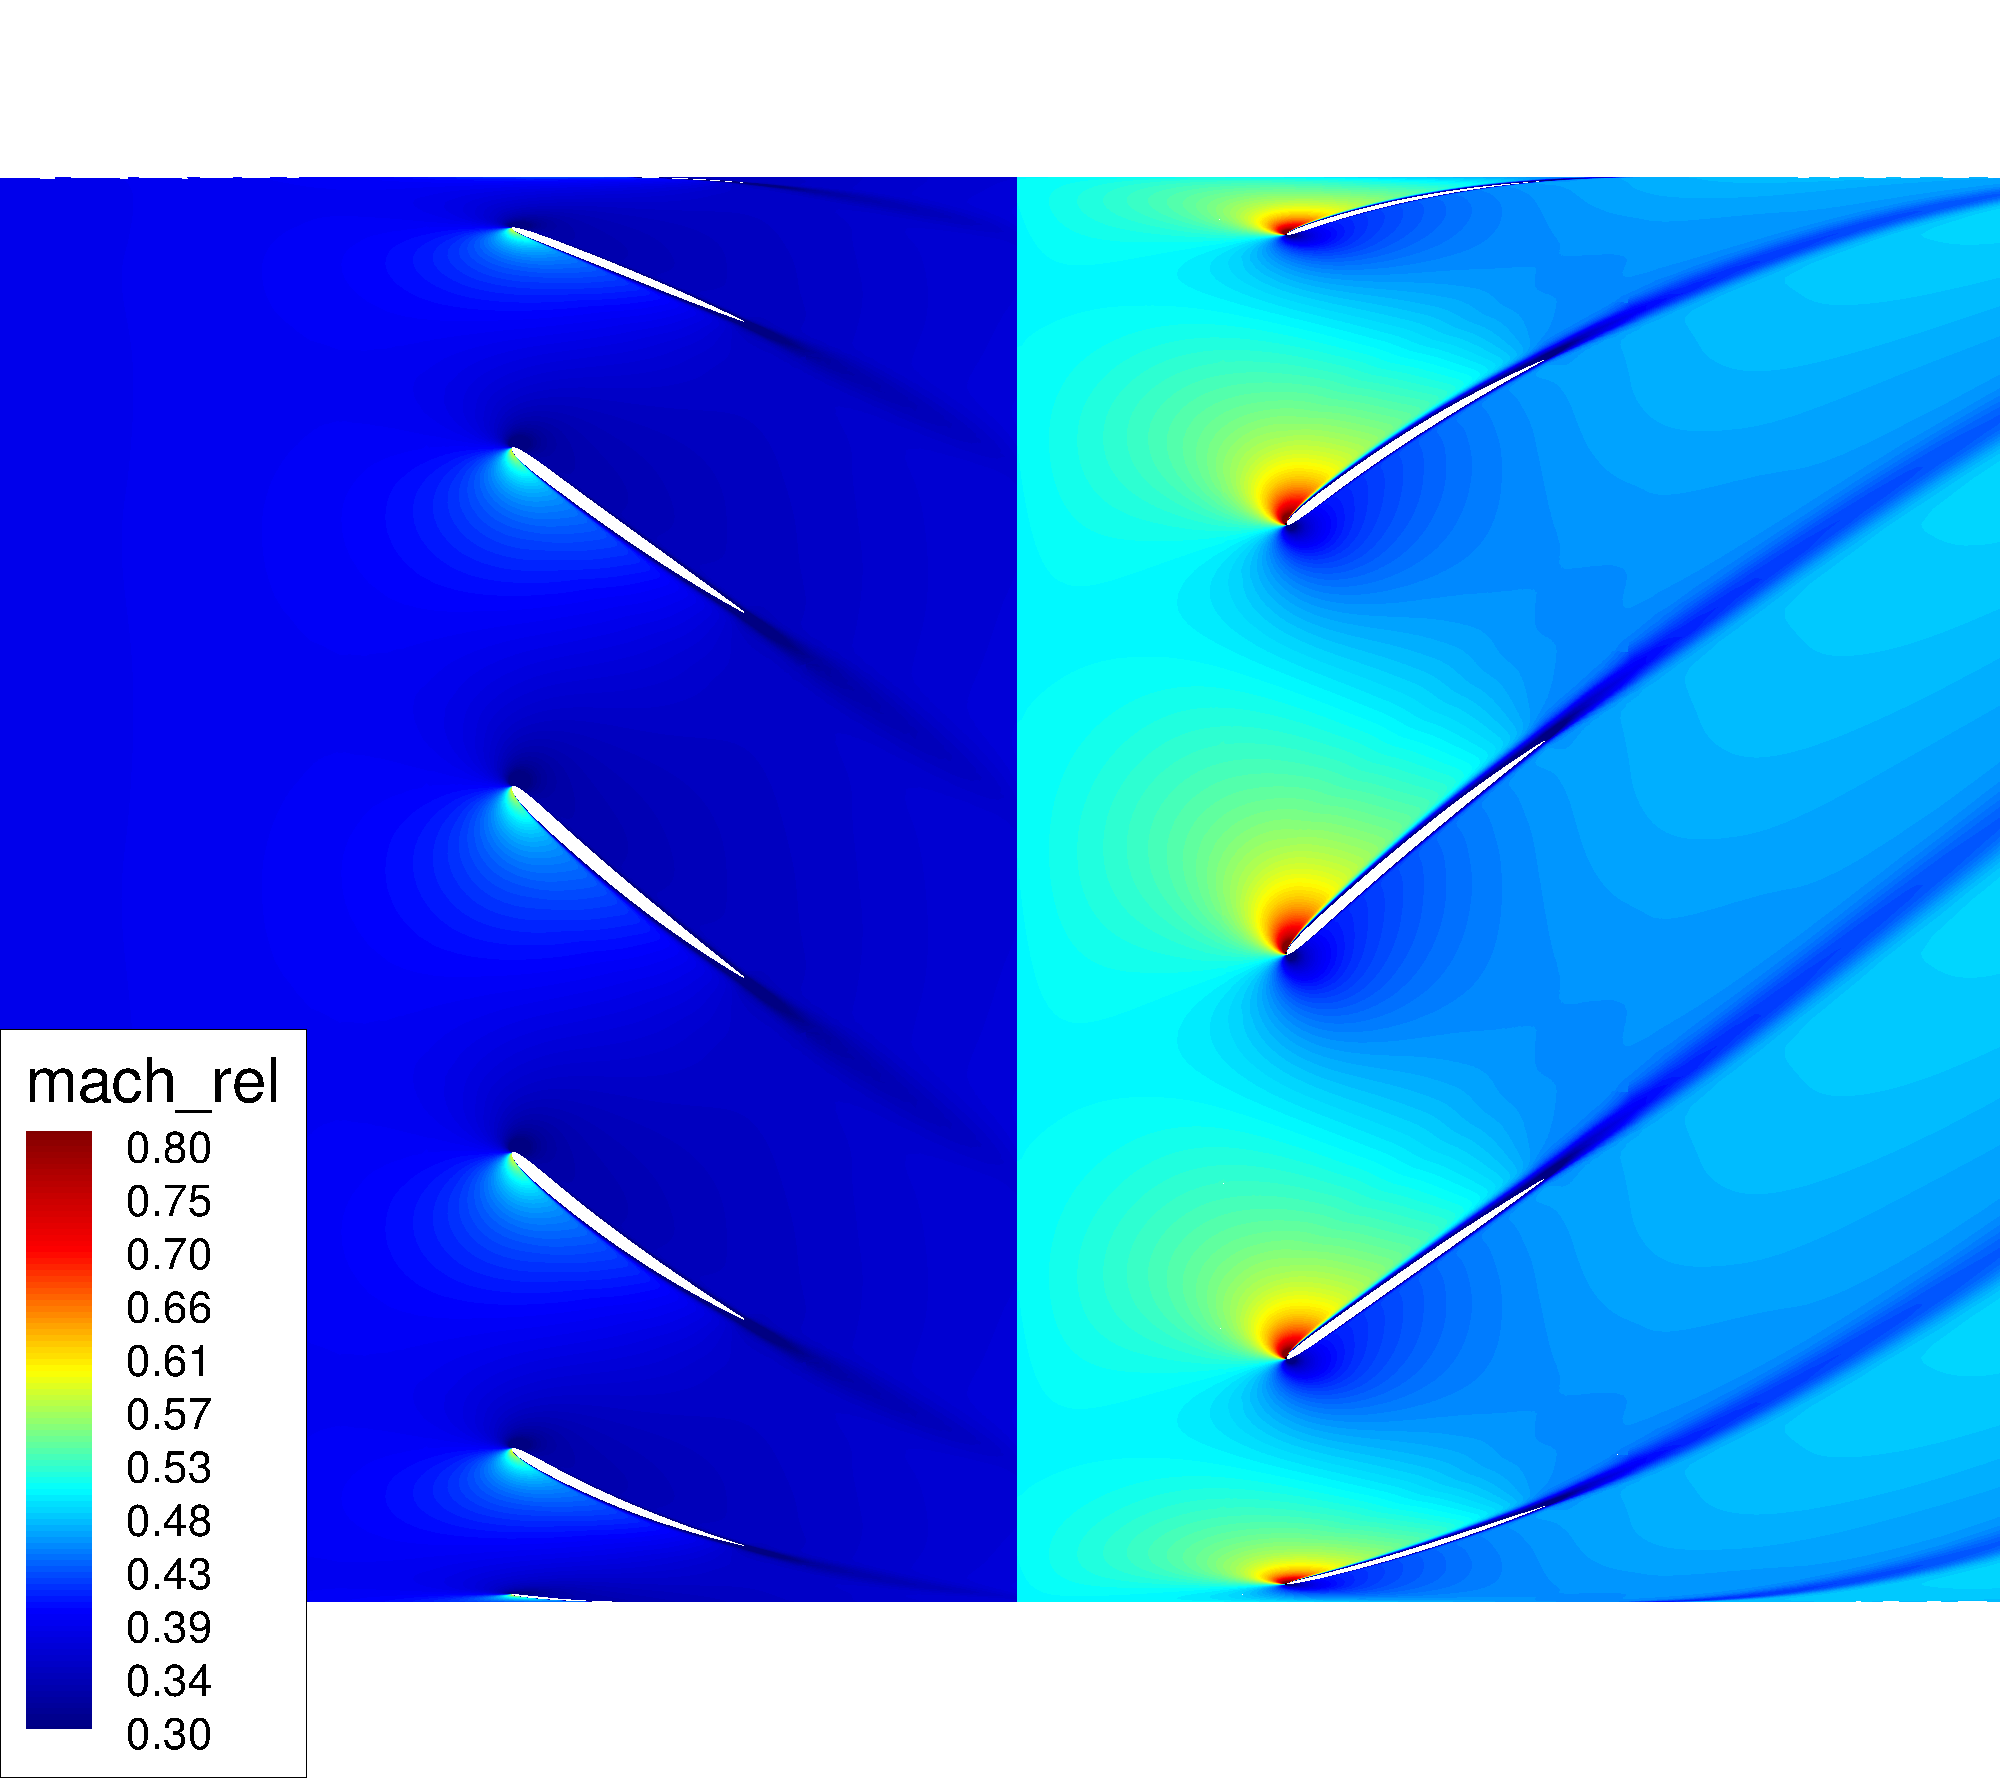
\includegraphics[width=0.28\textwidth]{DREAM_LS_RANS_roe2_sa_slice_r_25_mach_rel.png}\\
   \rotatebox{90}{\qquad\qquad 50~\%} 
   & 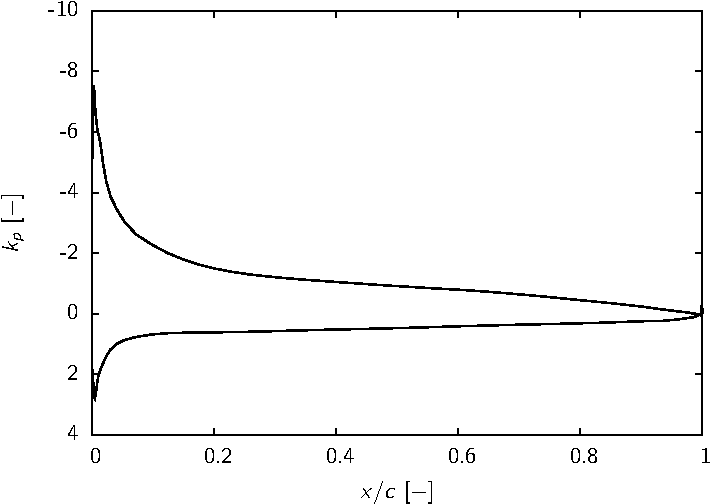
\includegraphics[width=0.28\textwidth]{DREAM_LS_KP_50_FRONT_PPT.pdf}
   & 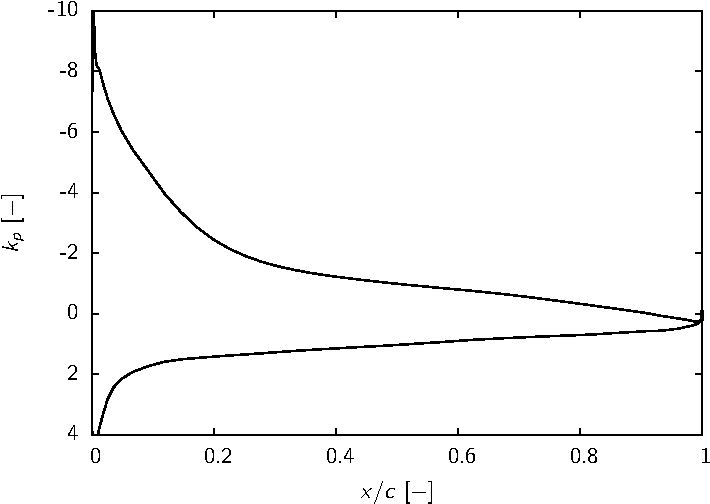
\includegraphics[width=0.28\textwidth]{DREAM_LS_KP_50_REAR_PPT.pdf}
   & 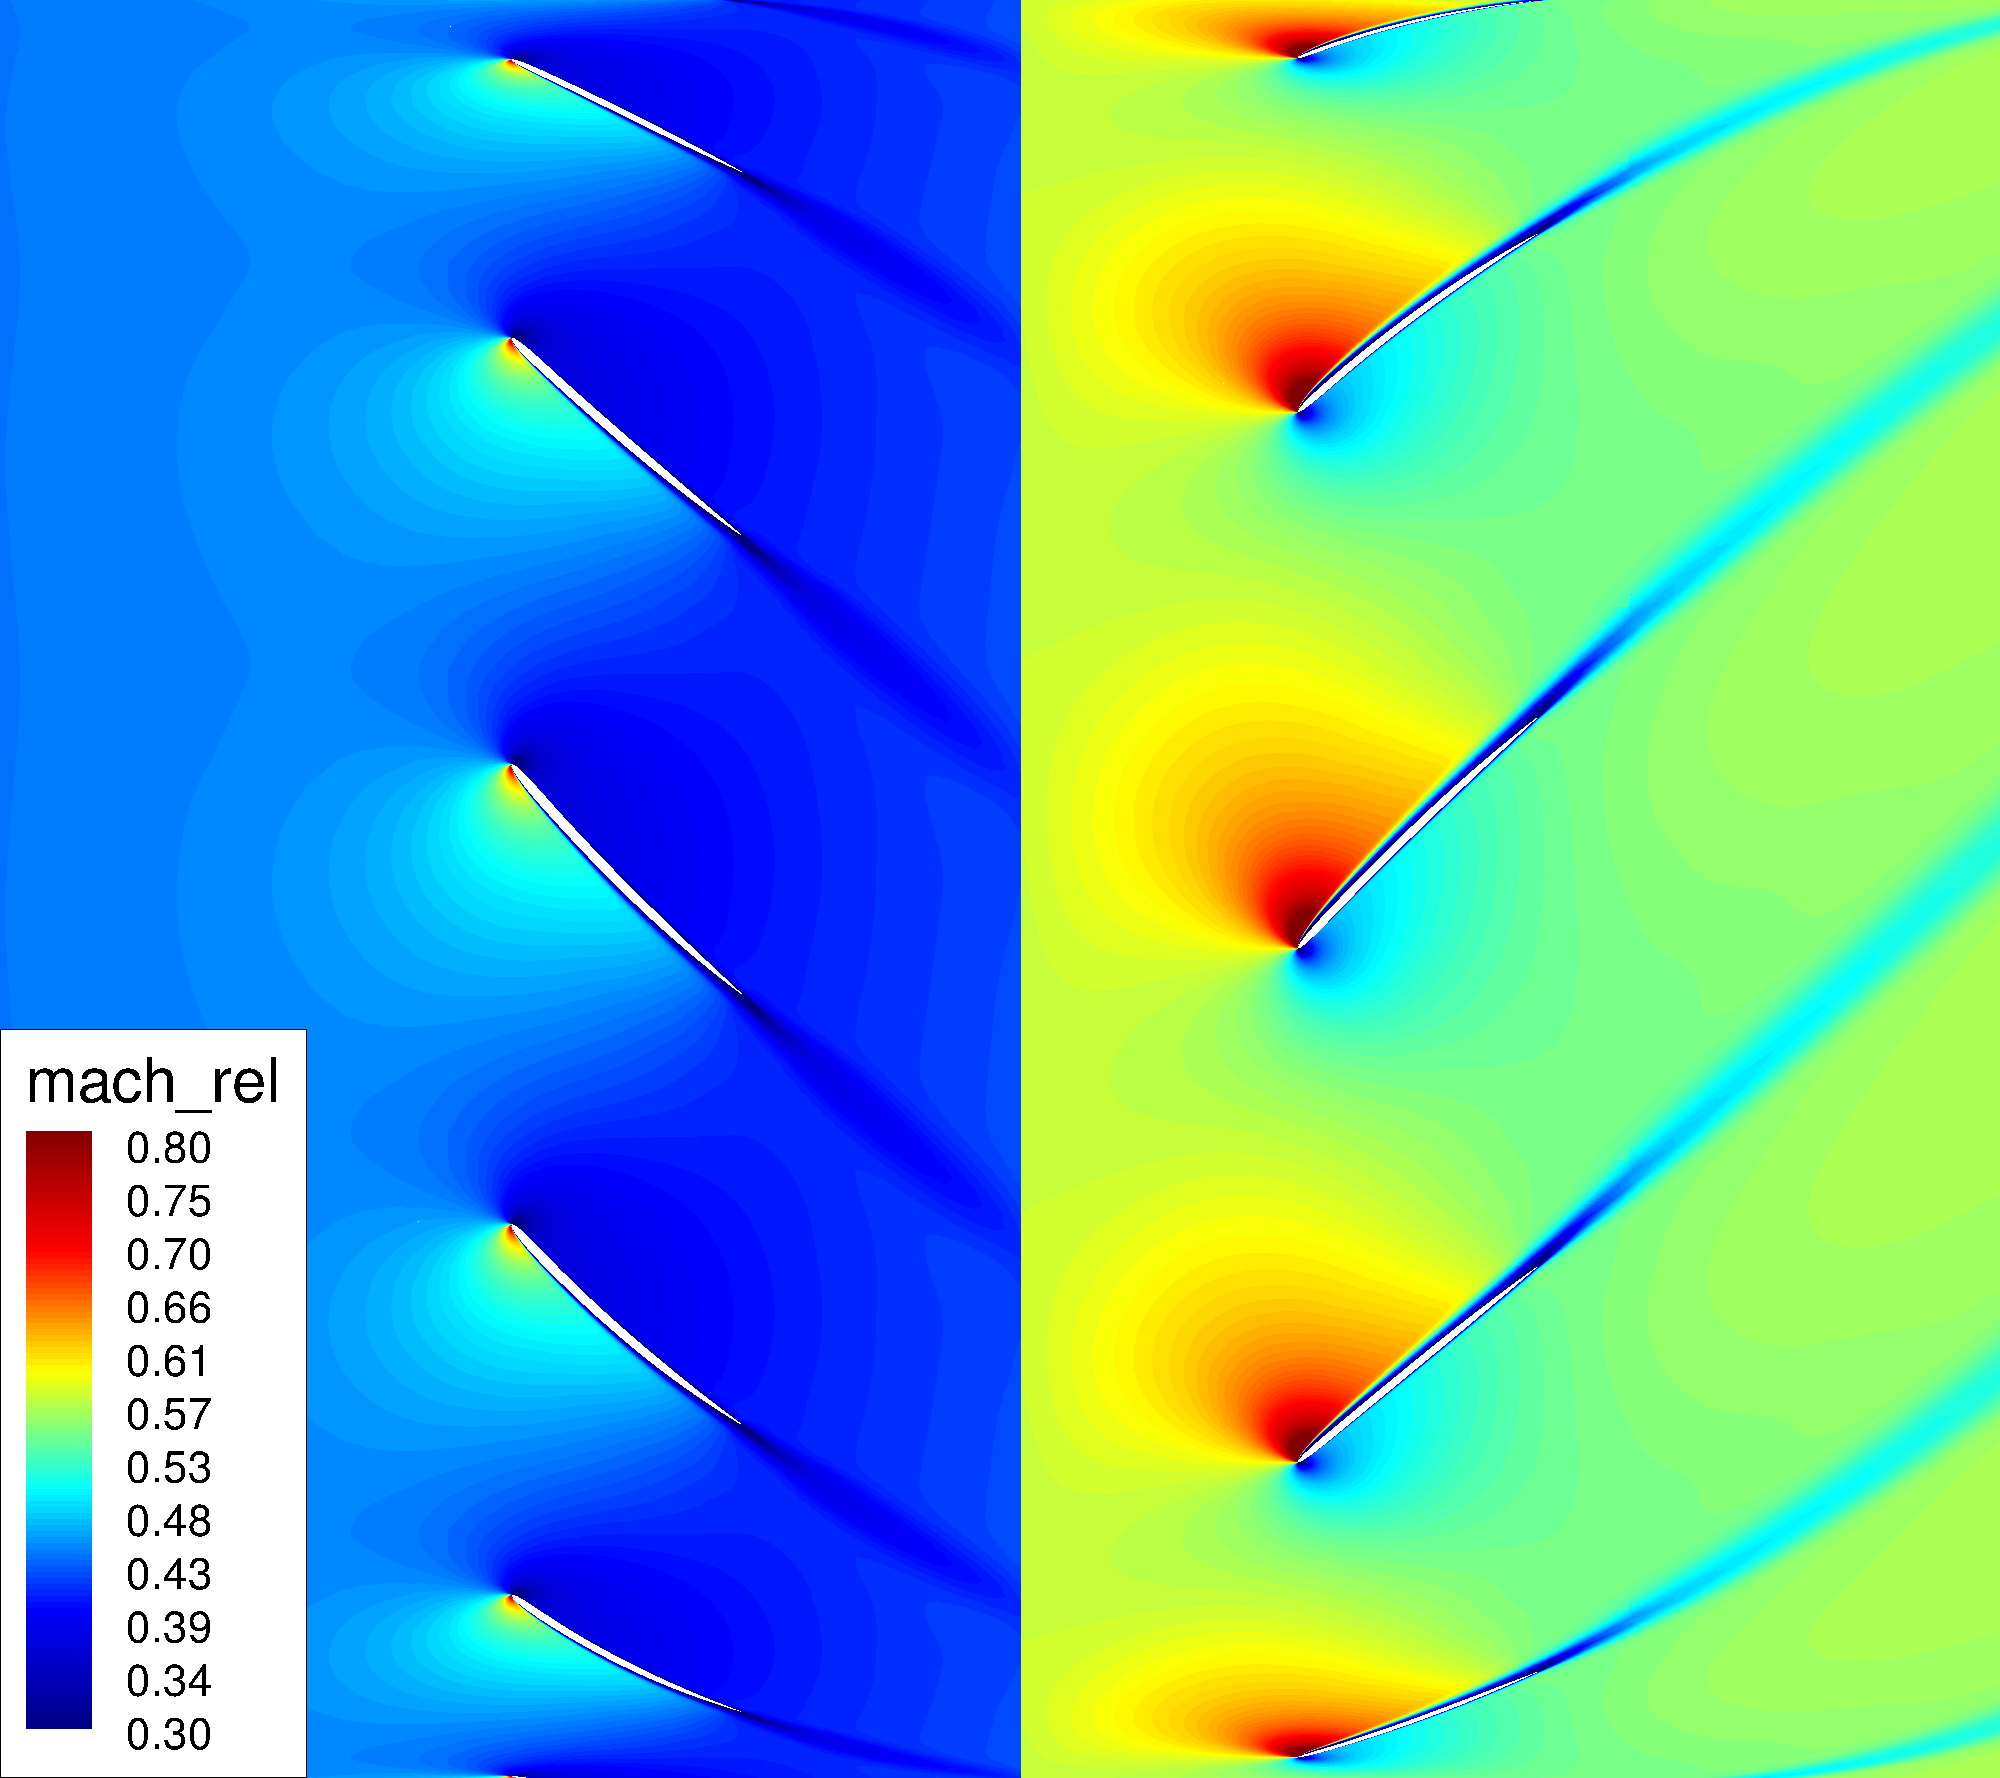
\includegraphics[width=0.28\textwidth]{DREAM_LS_RANS_roe2_sa_slice_r_50_mach_rel.png}\\
   \rotatebox{90}{\qquad\qquad 75~\%} 
   & 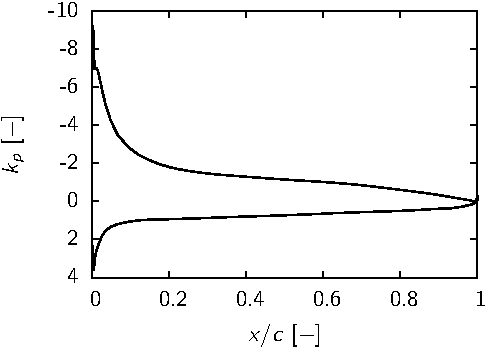
\includegraphics[width=0.28\textwidth]{DREAM_LS_KP_75_FRONT_PPT.pdf}
   & 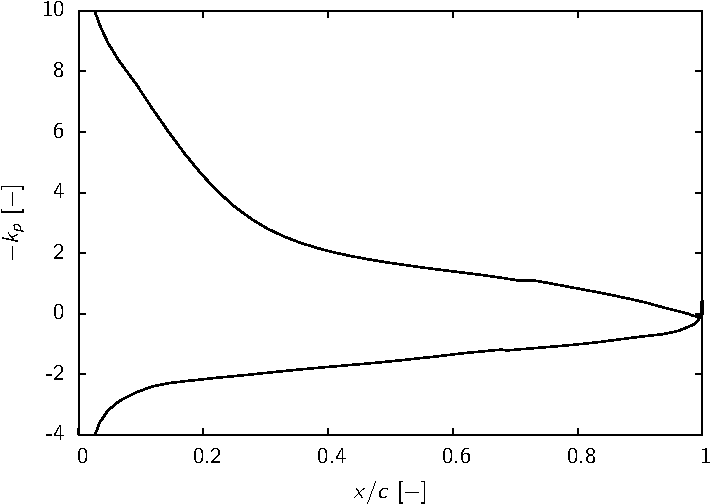
\includegraphics[width=0.28\textwidth]{DREAM_LS_KP_75_REAR_PPT.pdf}
   & 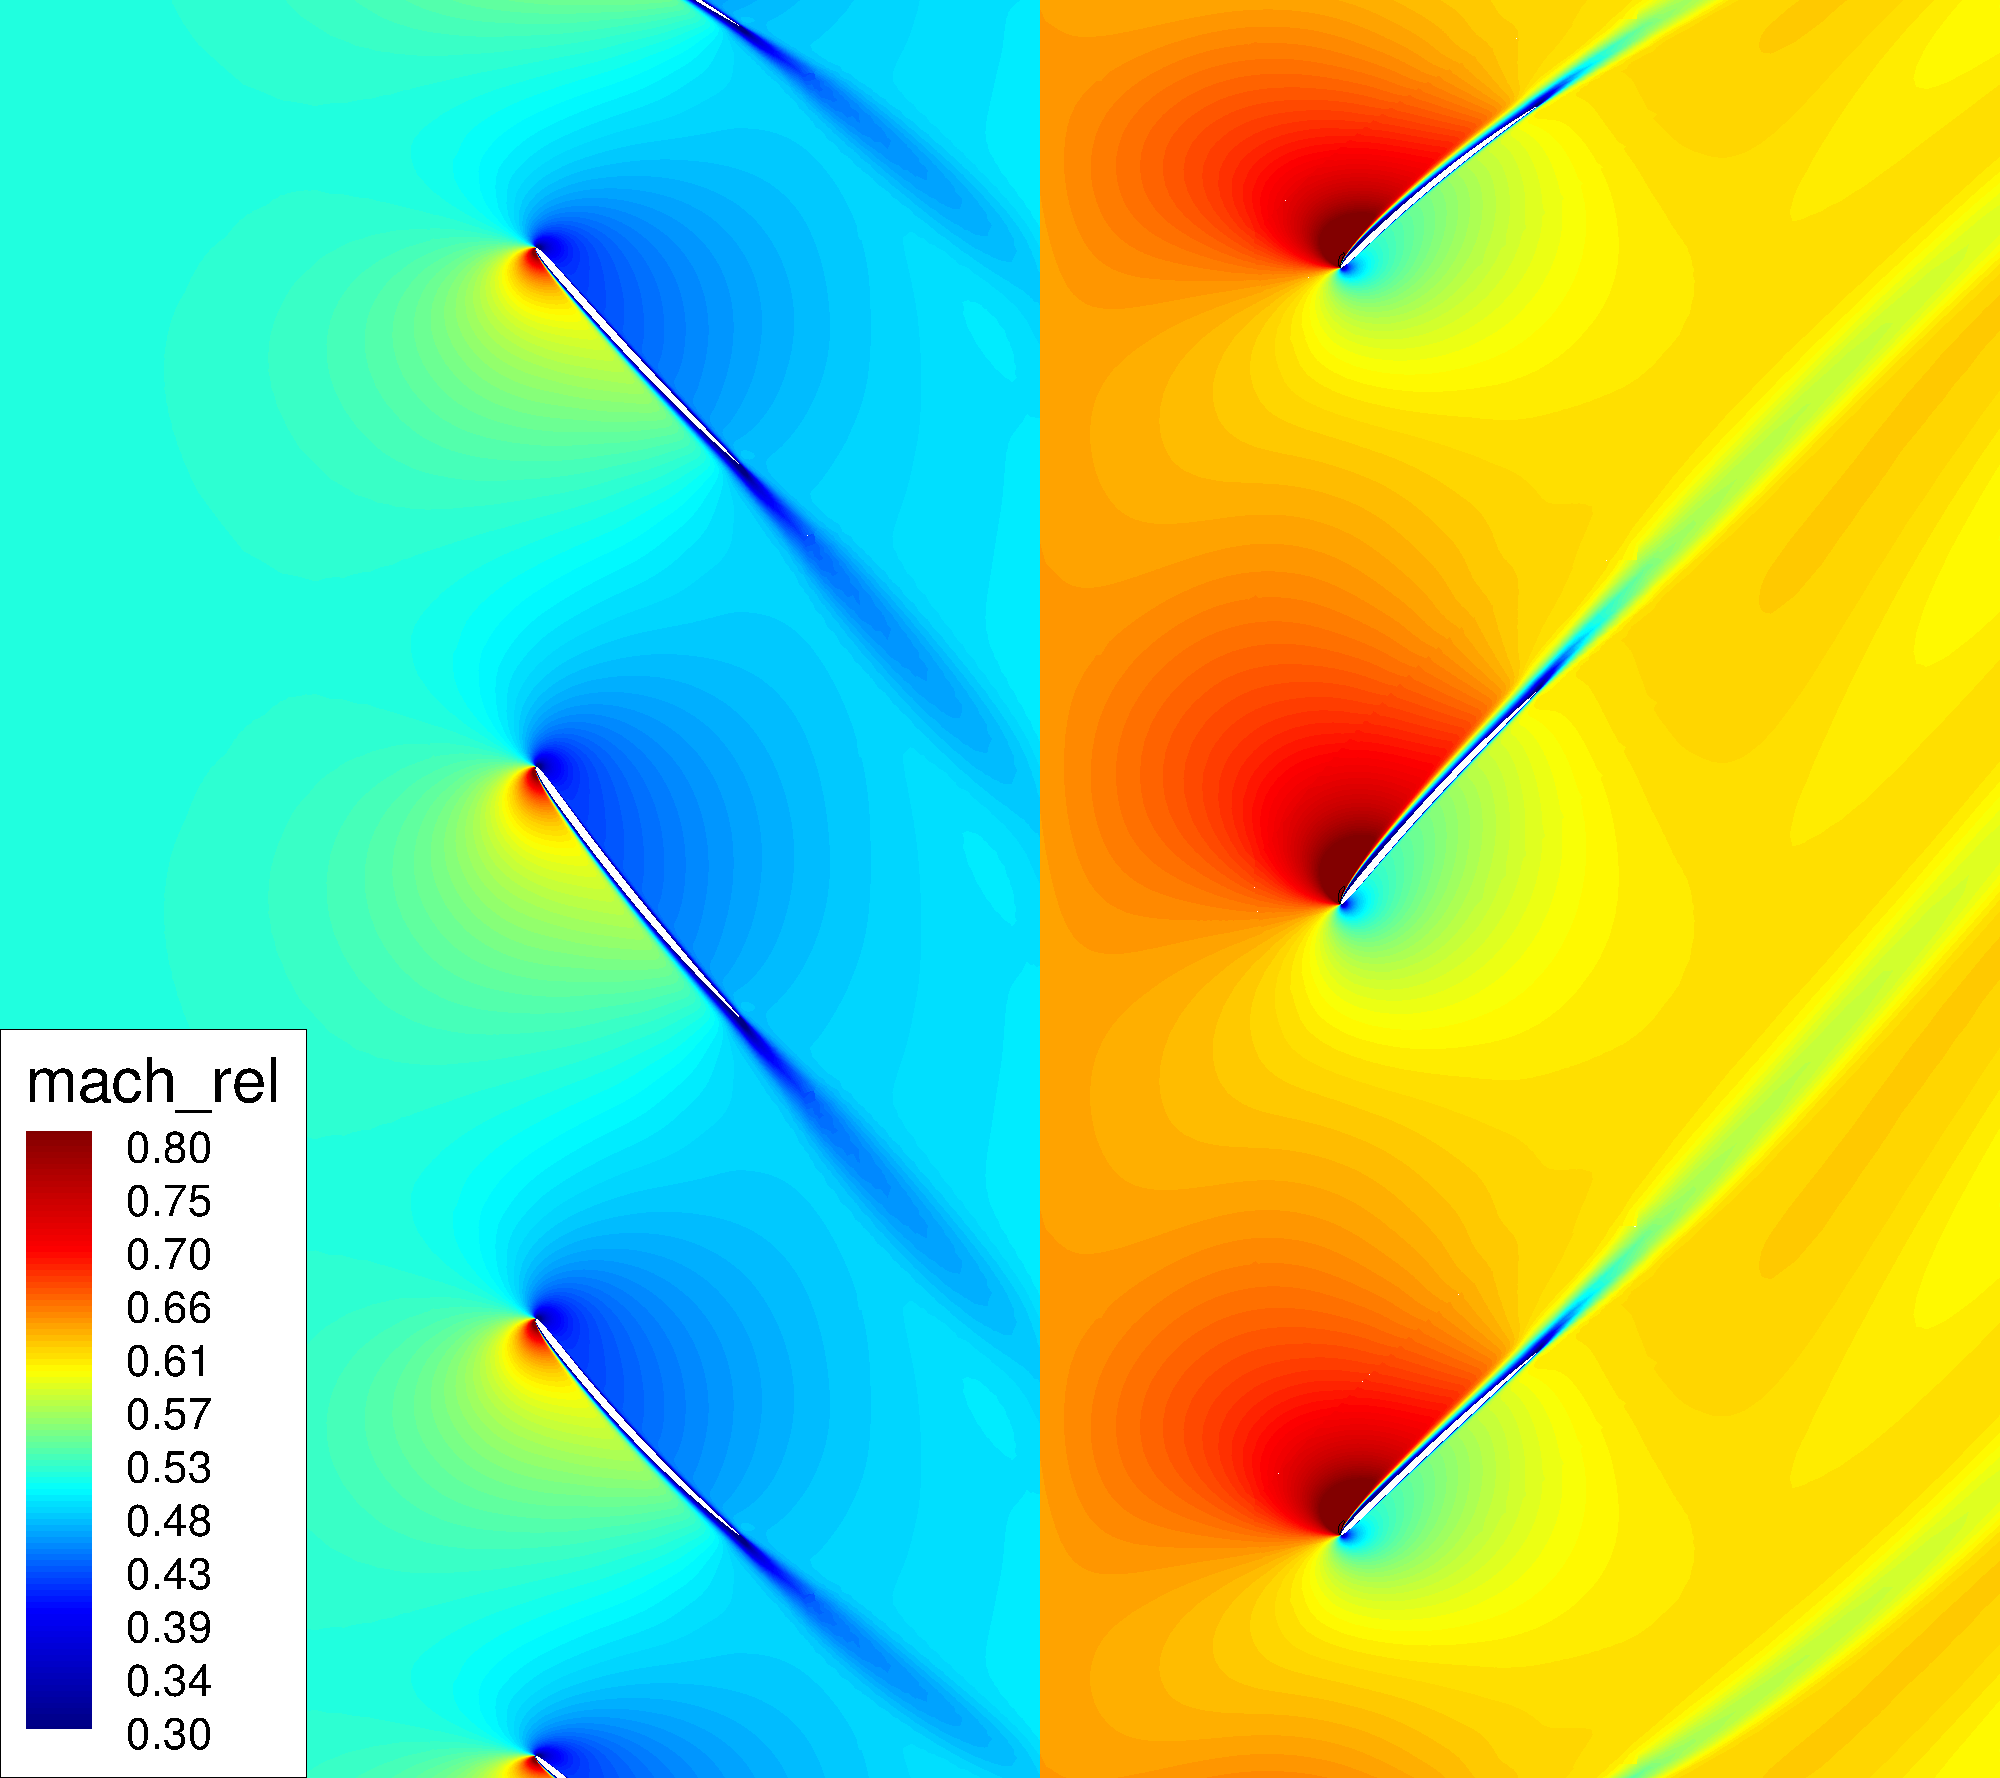
\includegraphics[width=0.28\textwidth]{DREAM_LS_RANS_roe2_sa_slice_r_75_mach_rel.png}\\
   \rotatebox{90}{\qquad\qquad 90~\%} 
   & 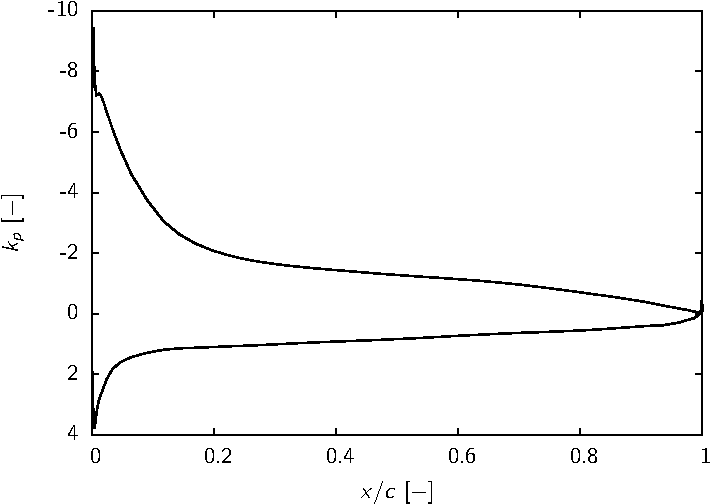
\includegraphics[width=0.28\textwidth]{DREAM_LS_KP_90_FRONT_PPT.pdf}
   & 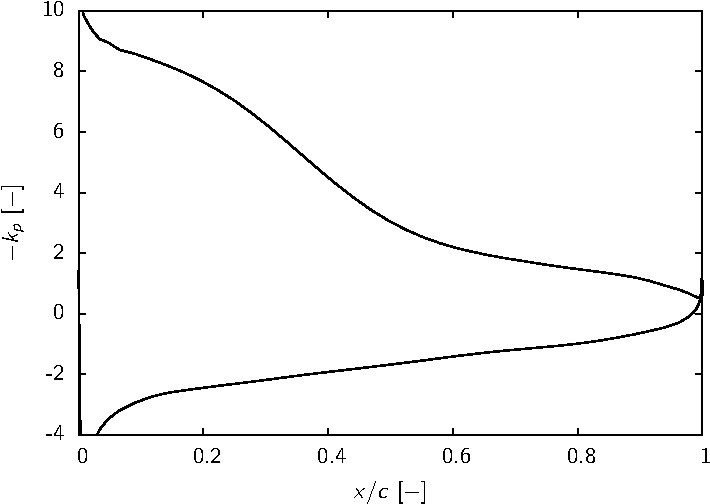
\includegraphics[width=0.28\textwidth]{DREAM_LS_KP_90_REAR_PPT.pdf}
   & 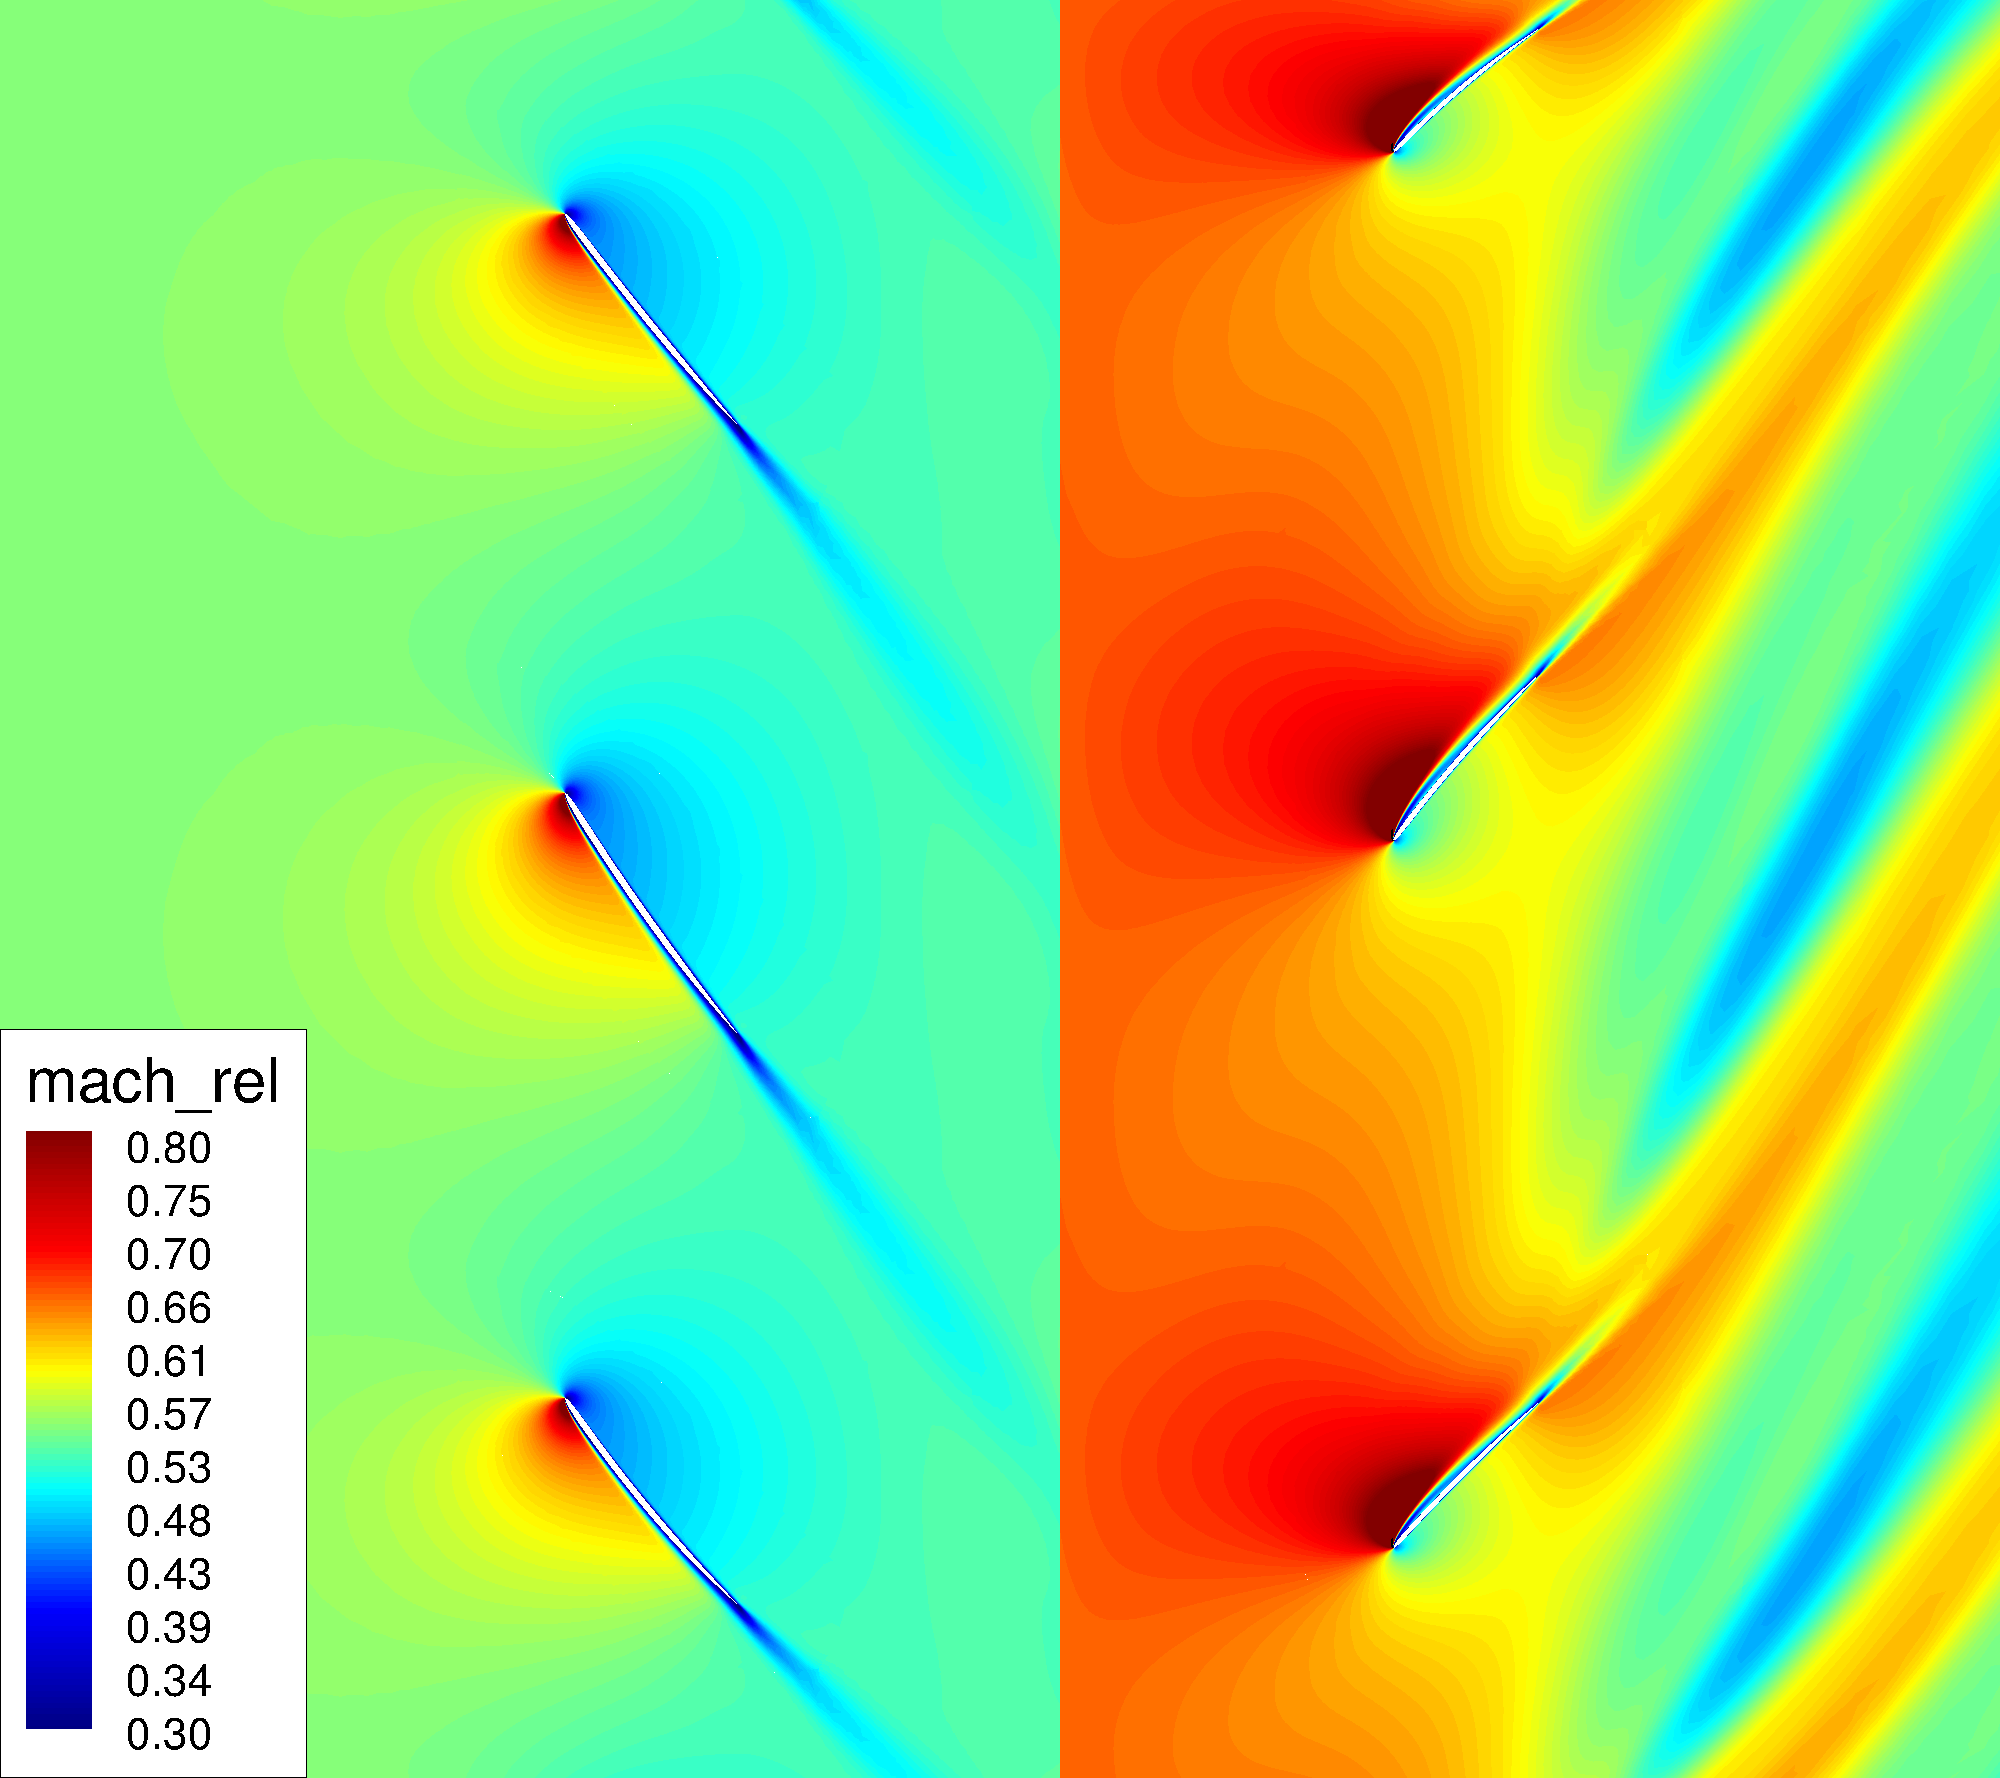
\includegraphics[width=0.28\textwidth]{DREAM_LS_RANS_roe2_sa_slice_r_90_mach_rel.png}\\
   \rotatebox{90}{\qquad\qquad 95~\%} 
   & 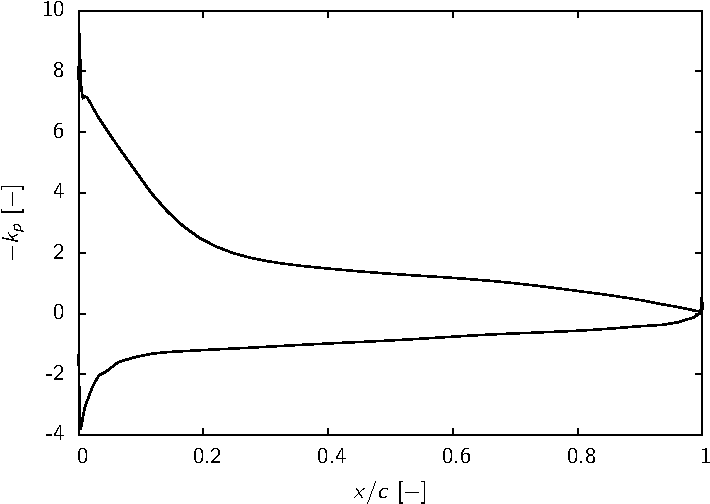
\includegraphics[width=0.28\textwidth]{DREAM_LS_KP_95_FRONT_PPT.pdf}
   & 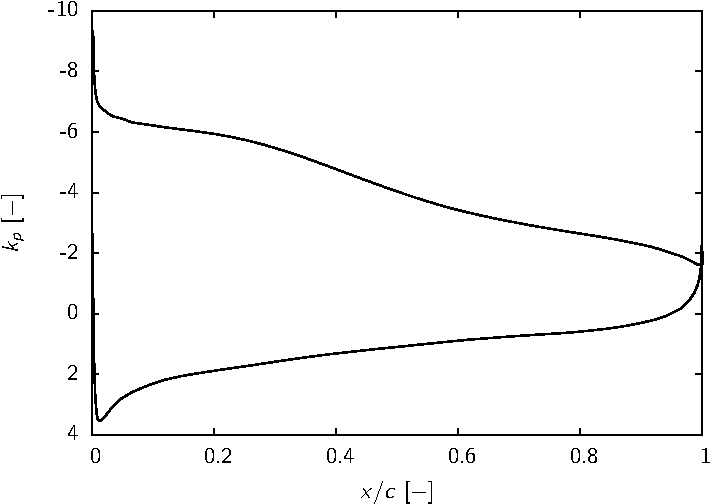
\includegraphics[width=0.28\textwidth]{DREAM_LS_KP_95_REAR_PPT.pdf}
   & 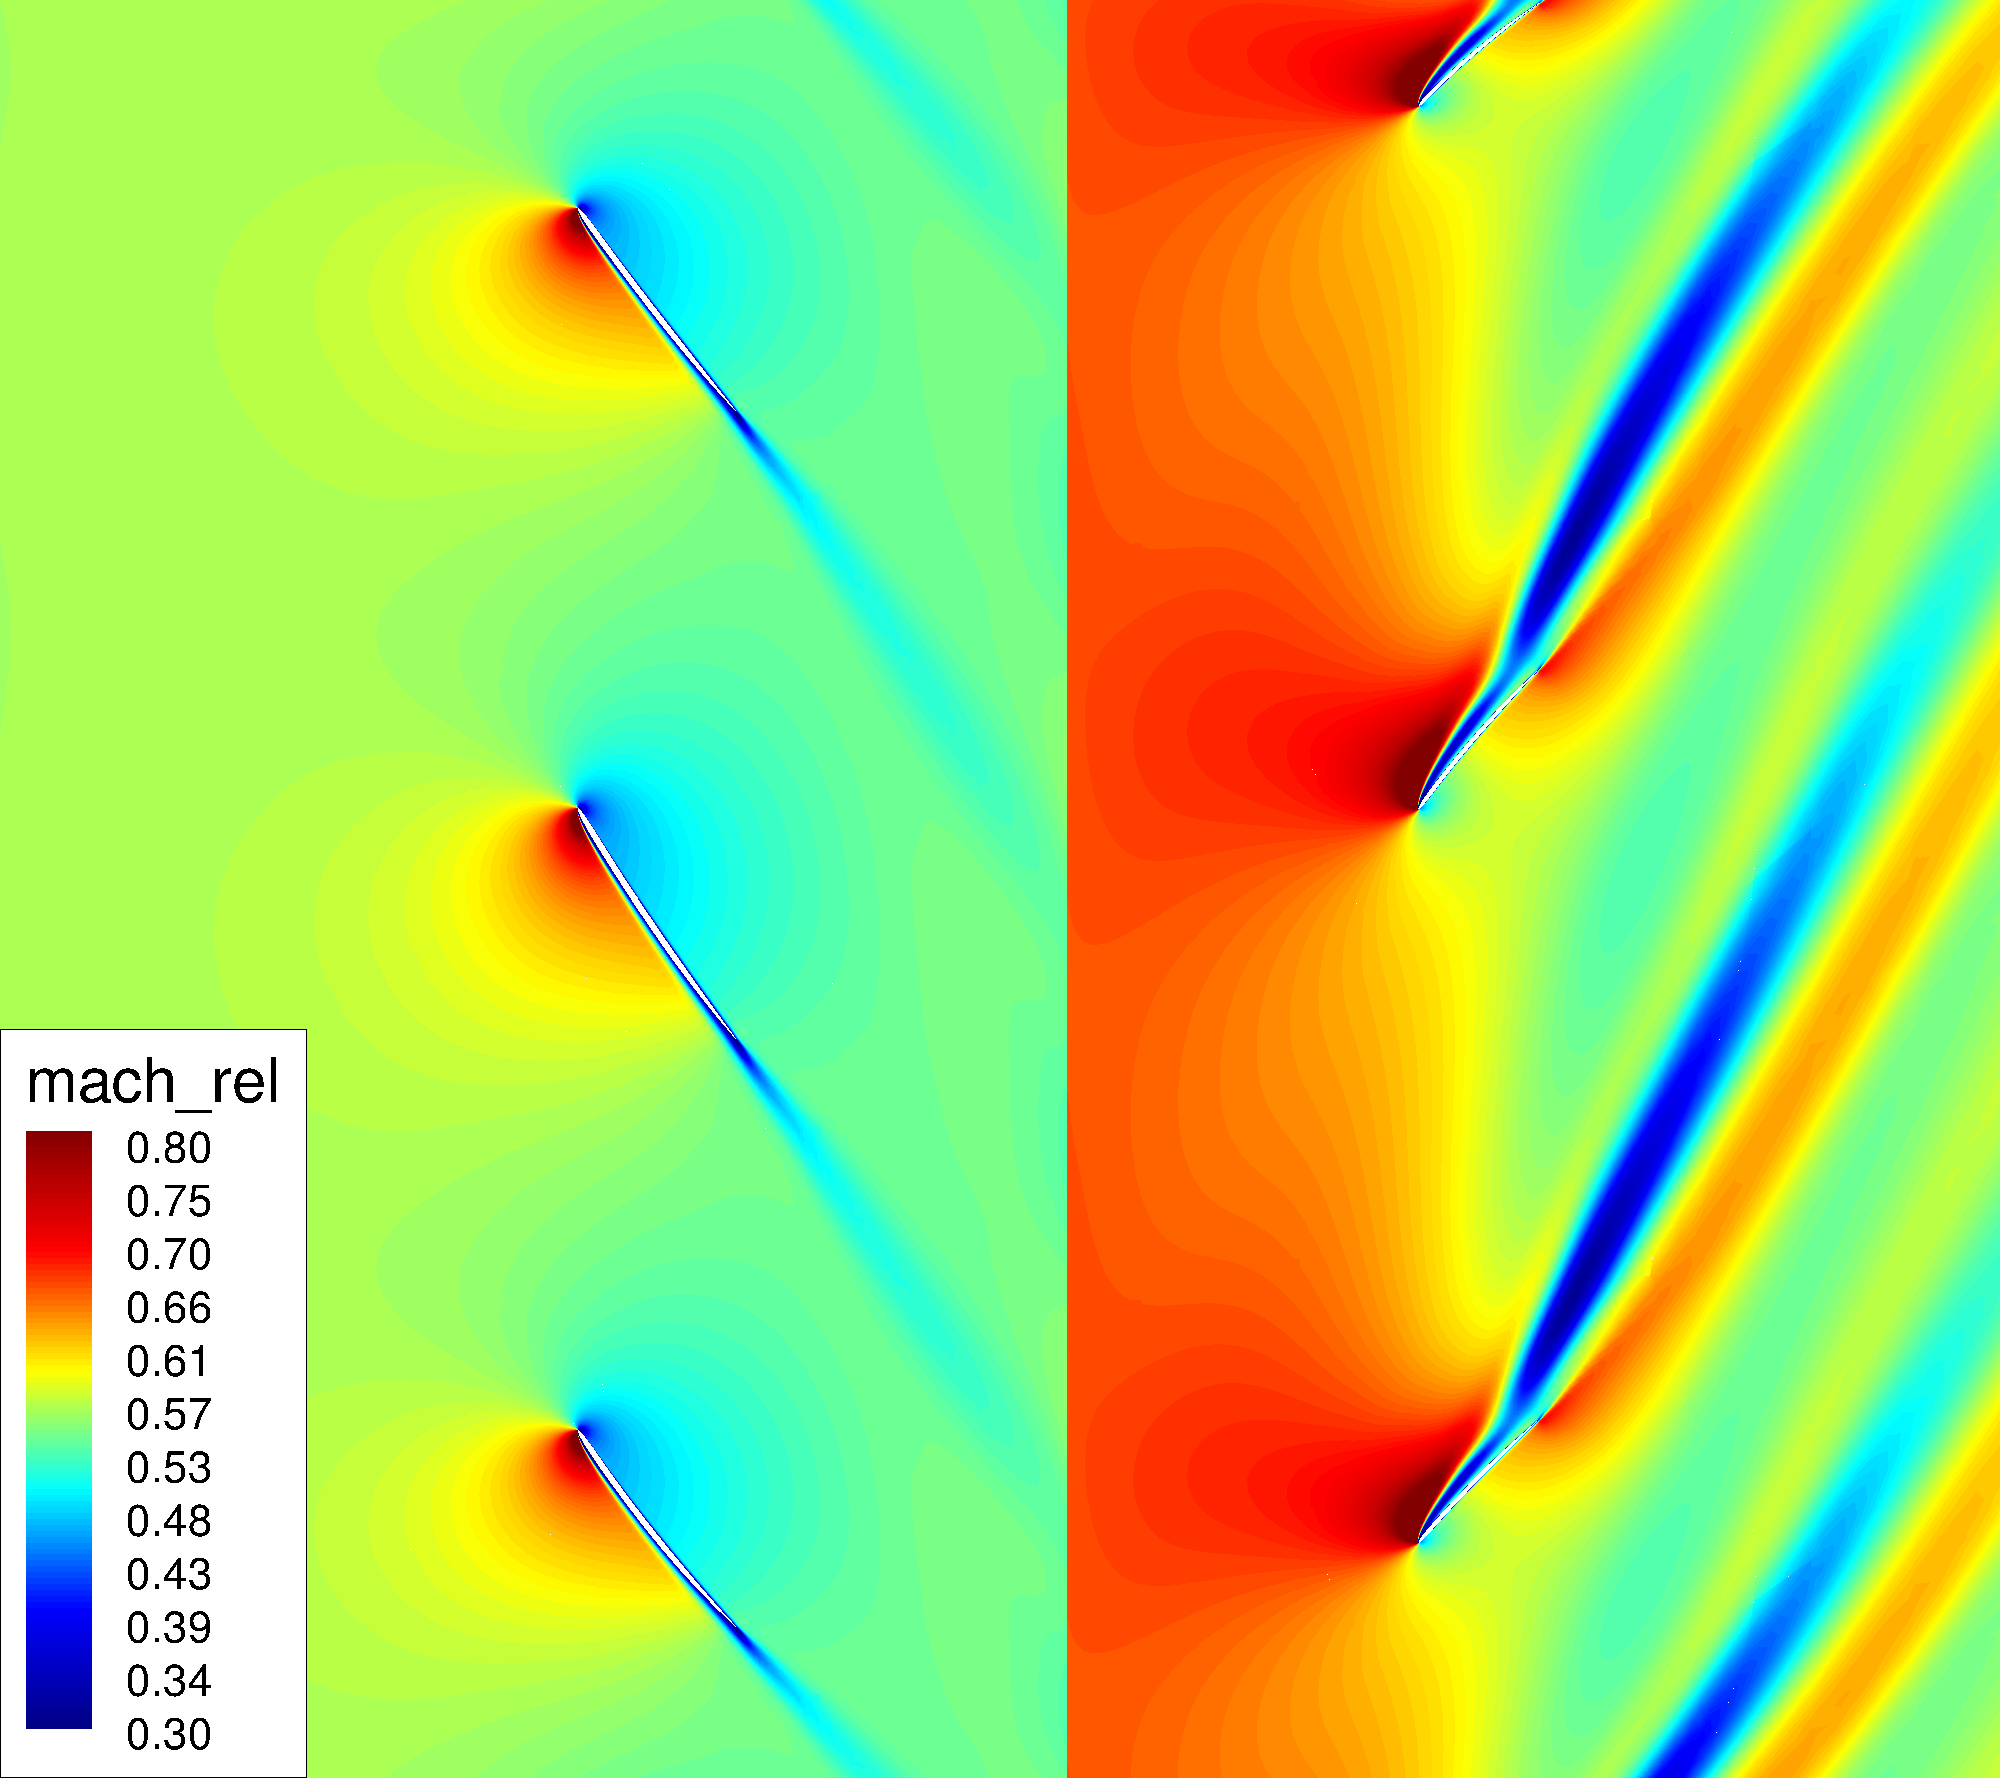
\includegraphics[width=0.28\textwidth]{DREAM_LS_RANS_roe2_sa_slice_r_95_mach_rel.png}  
 \end{tabular}
 \caption{Low-speed isolated configuration: pressure coefficient and relative Mach
 number contours at different radial position.}
 \label{fig:dream_ls_mach_kp}
\end{figure}

\begin{figure}[htb]
  \centering
  \subfigure[$P3$]{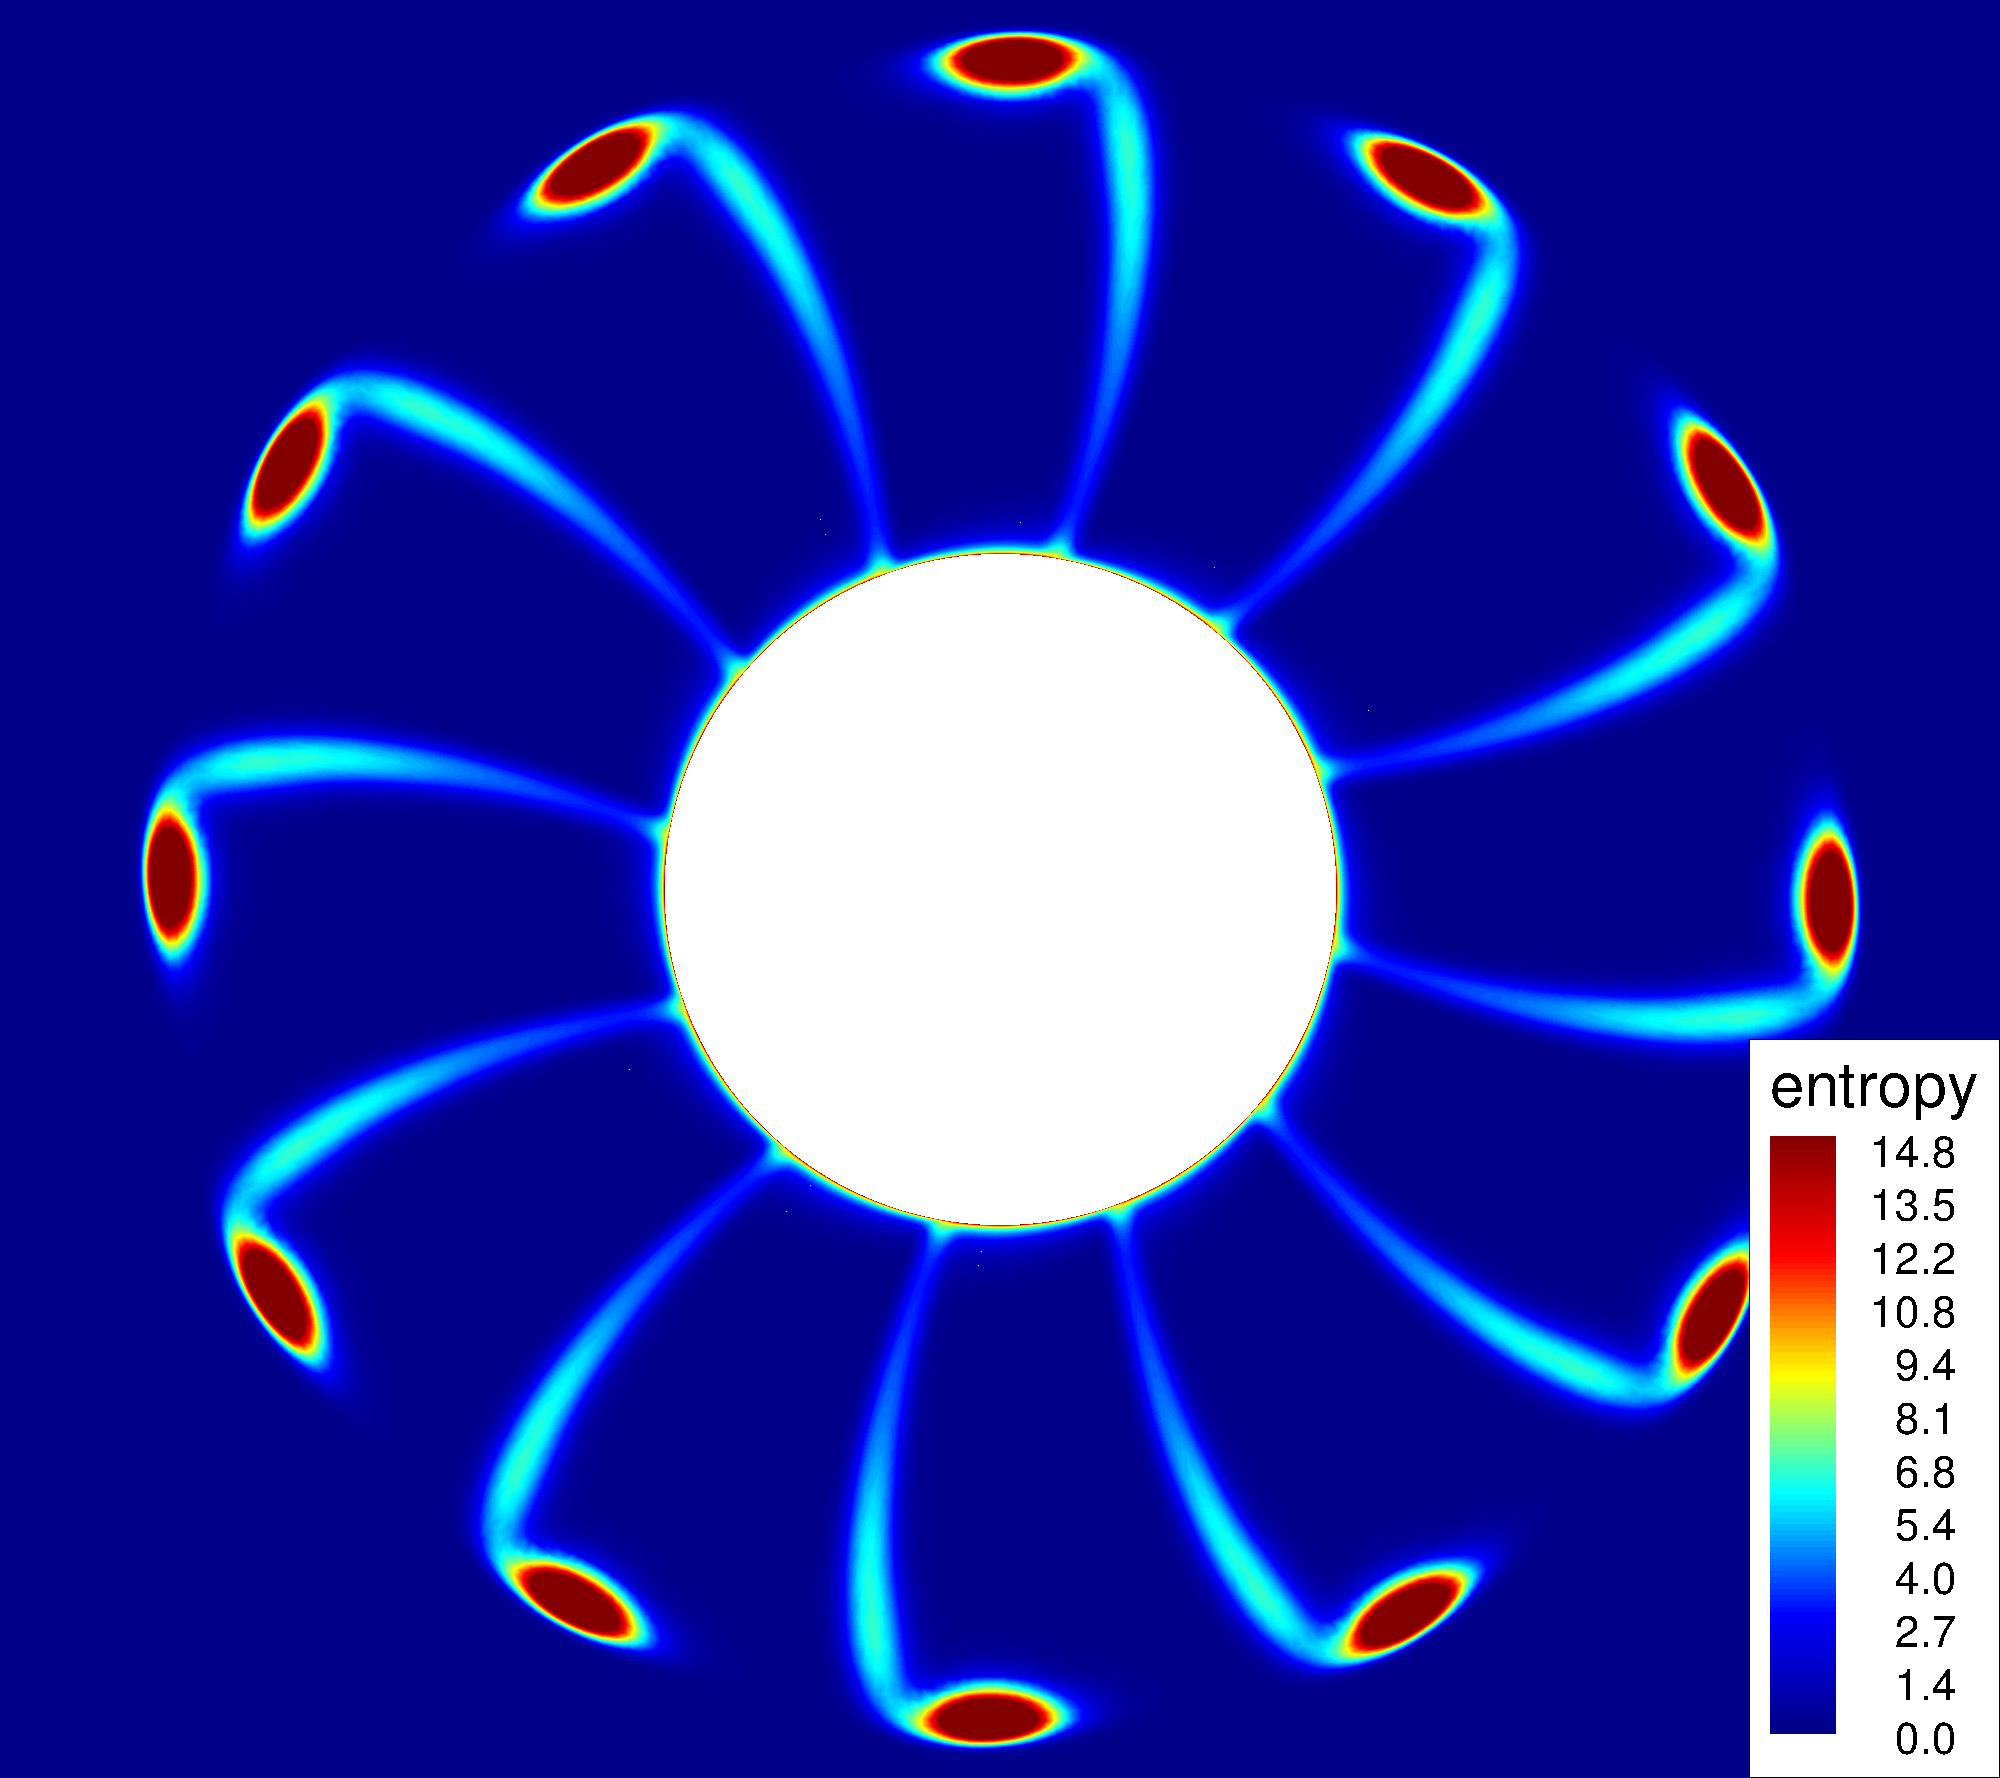
\includegraphics[width=.35\textwidth]{DREAM_LS_RANS_roe2_sa_slice_x_front_1_entropy.png}}
  \subfigure[$P4$]{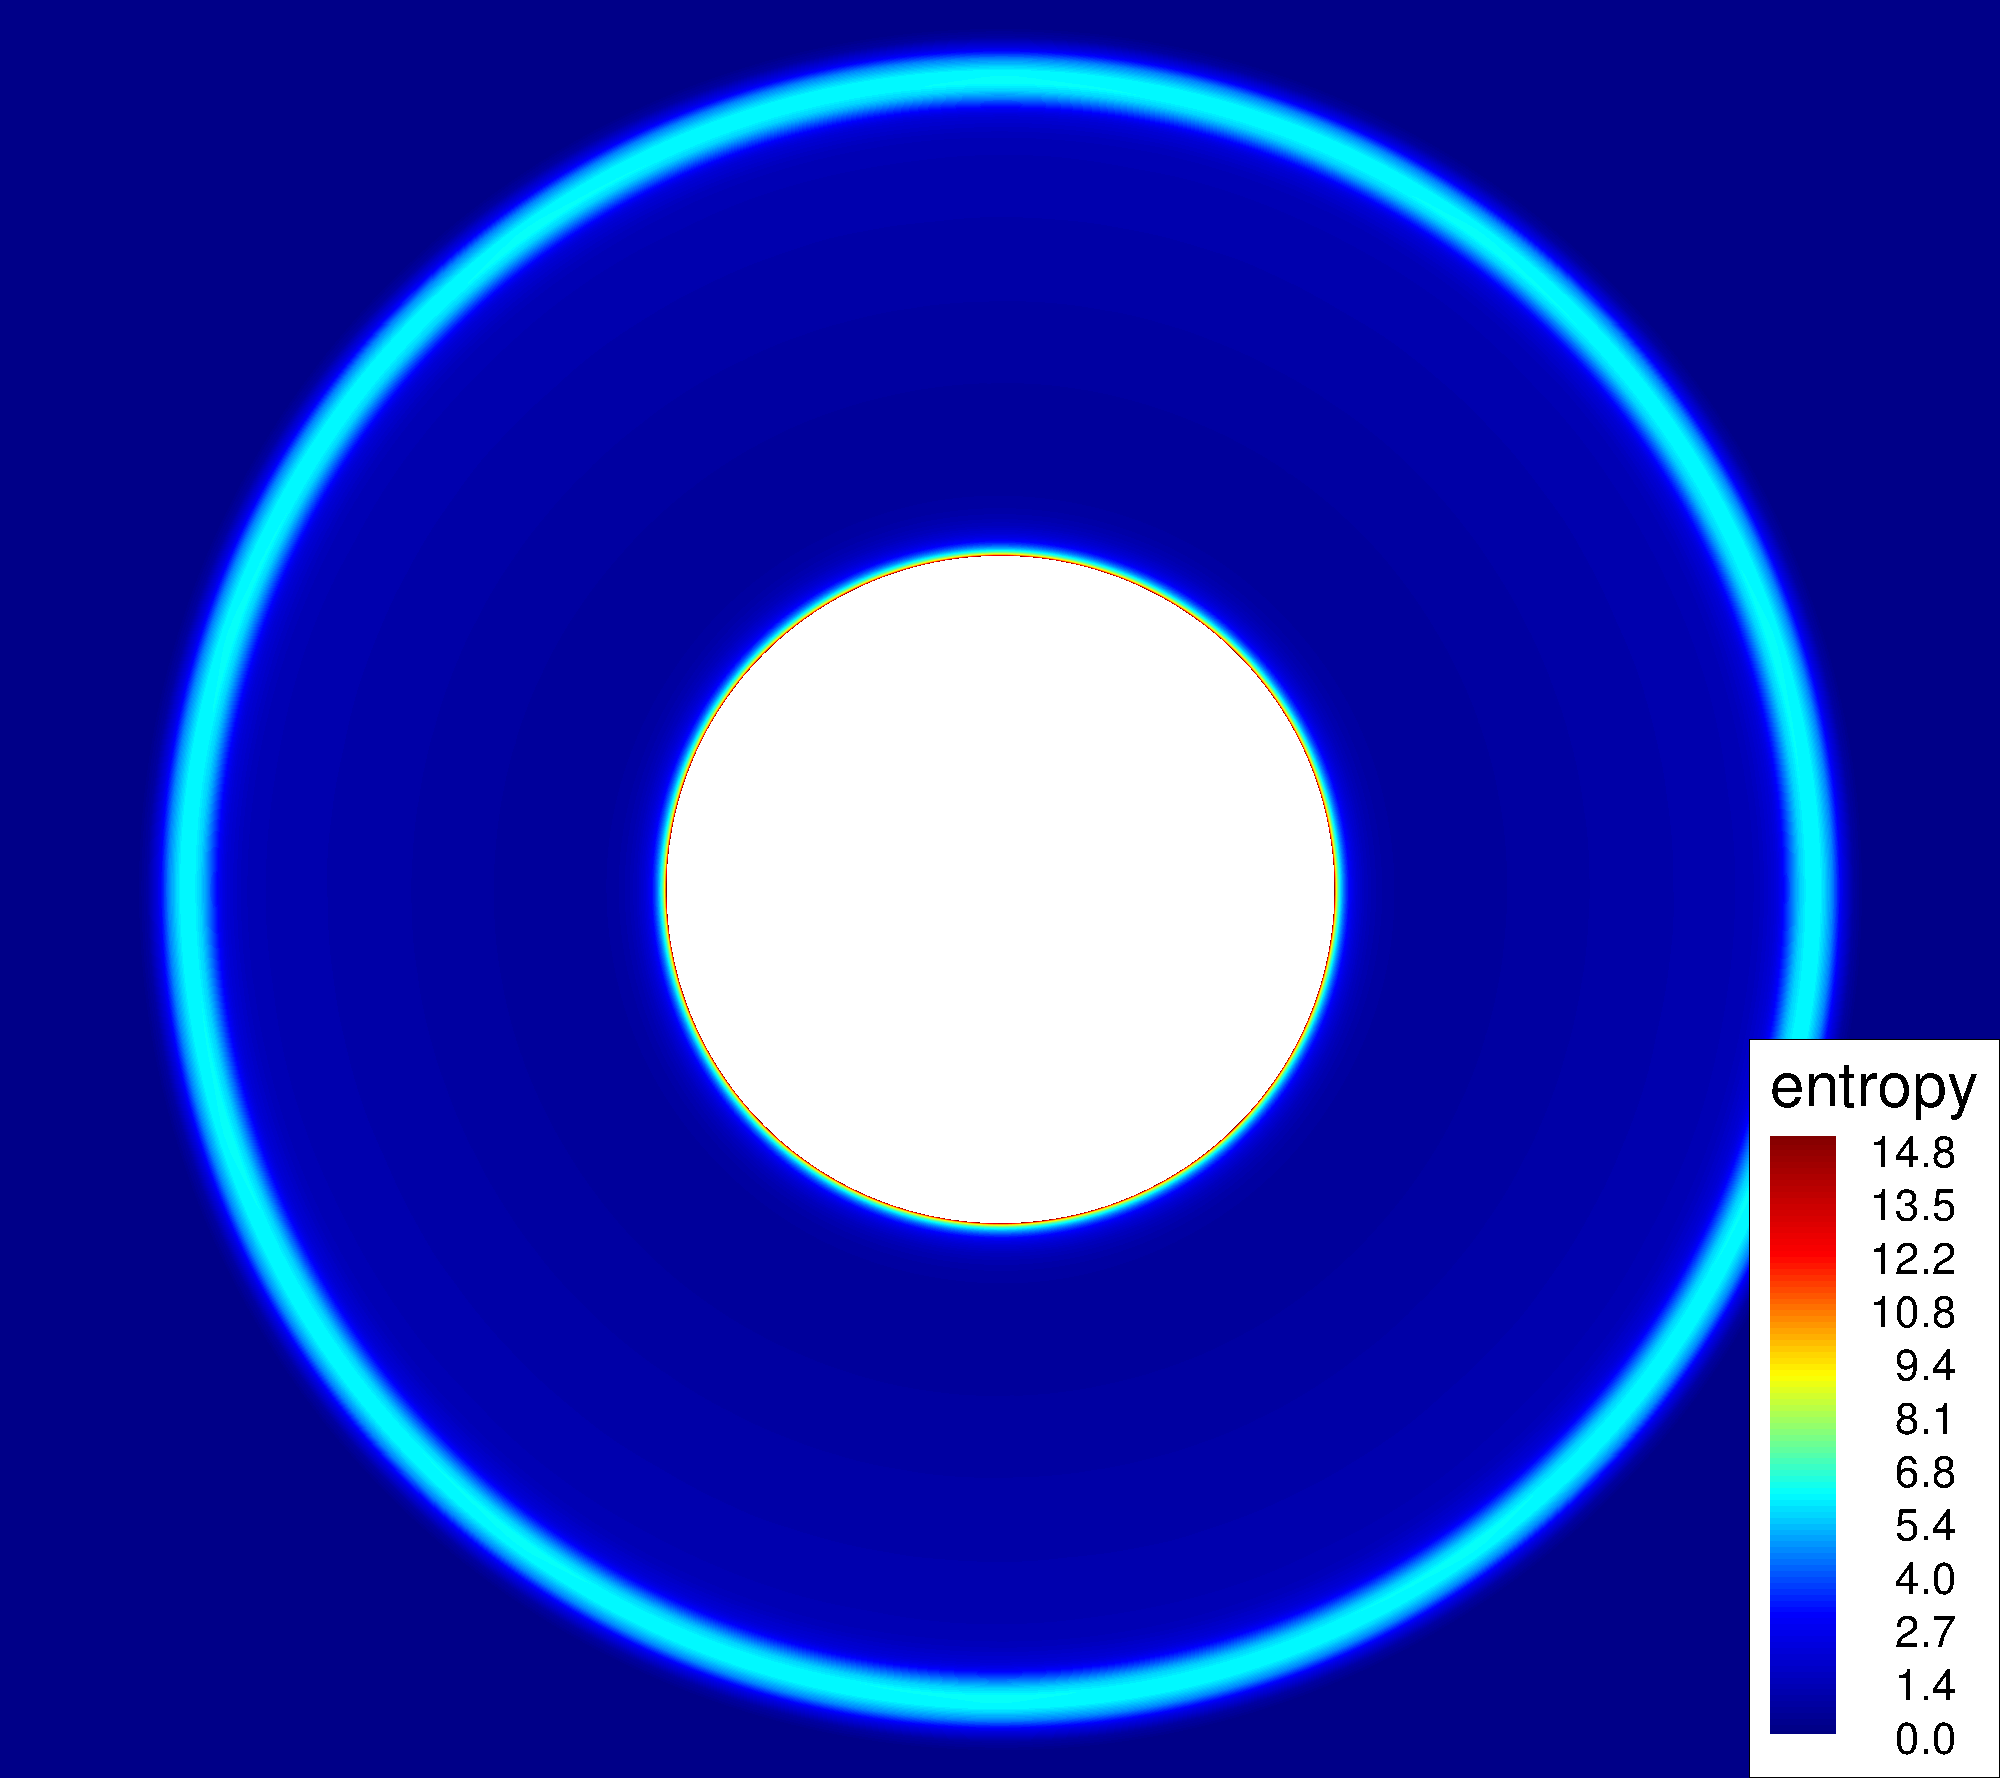
\includegraphics[width=.35\textwidth]{DREAM_LS_RANS_roe2_sa_slice_x_rear_-1_entropy.png}}
  \subfigure[$P5$]{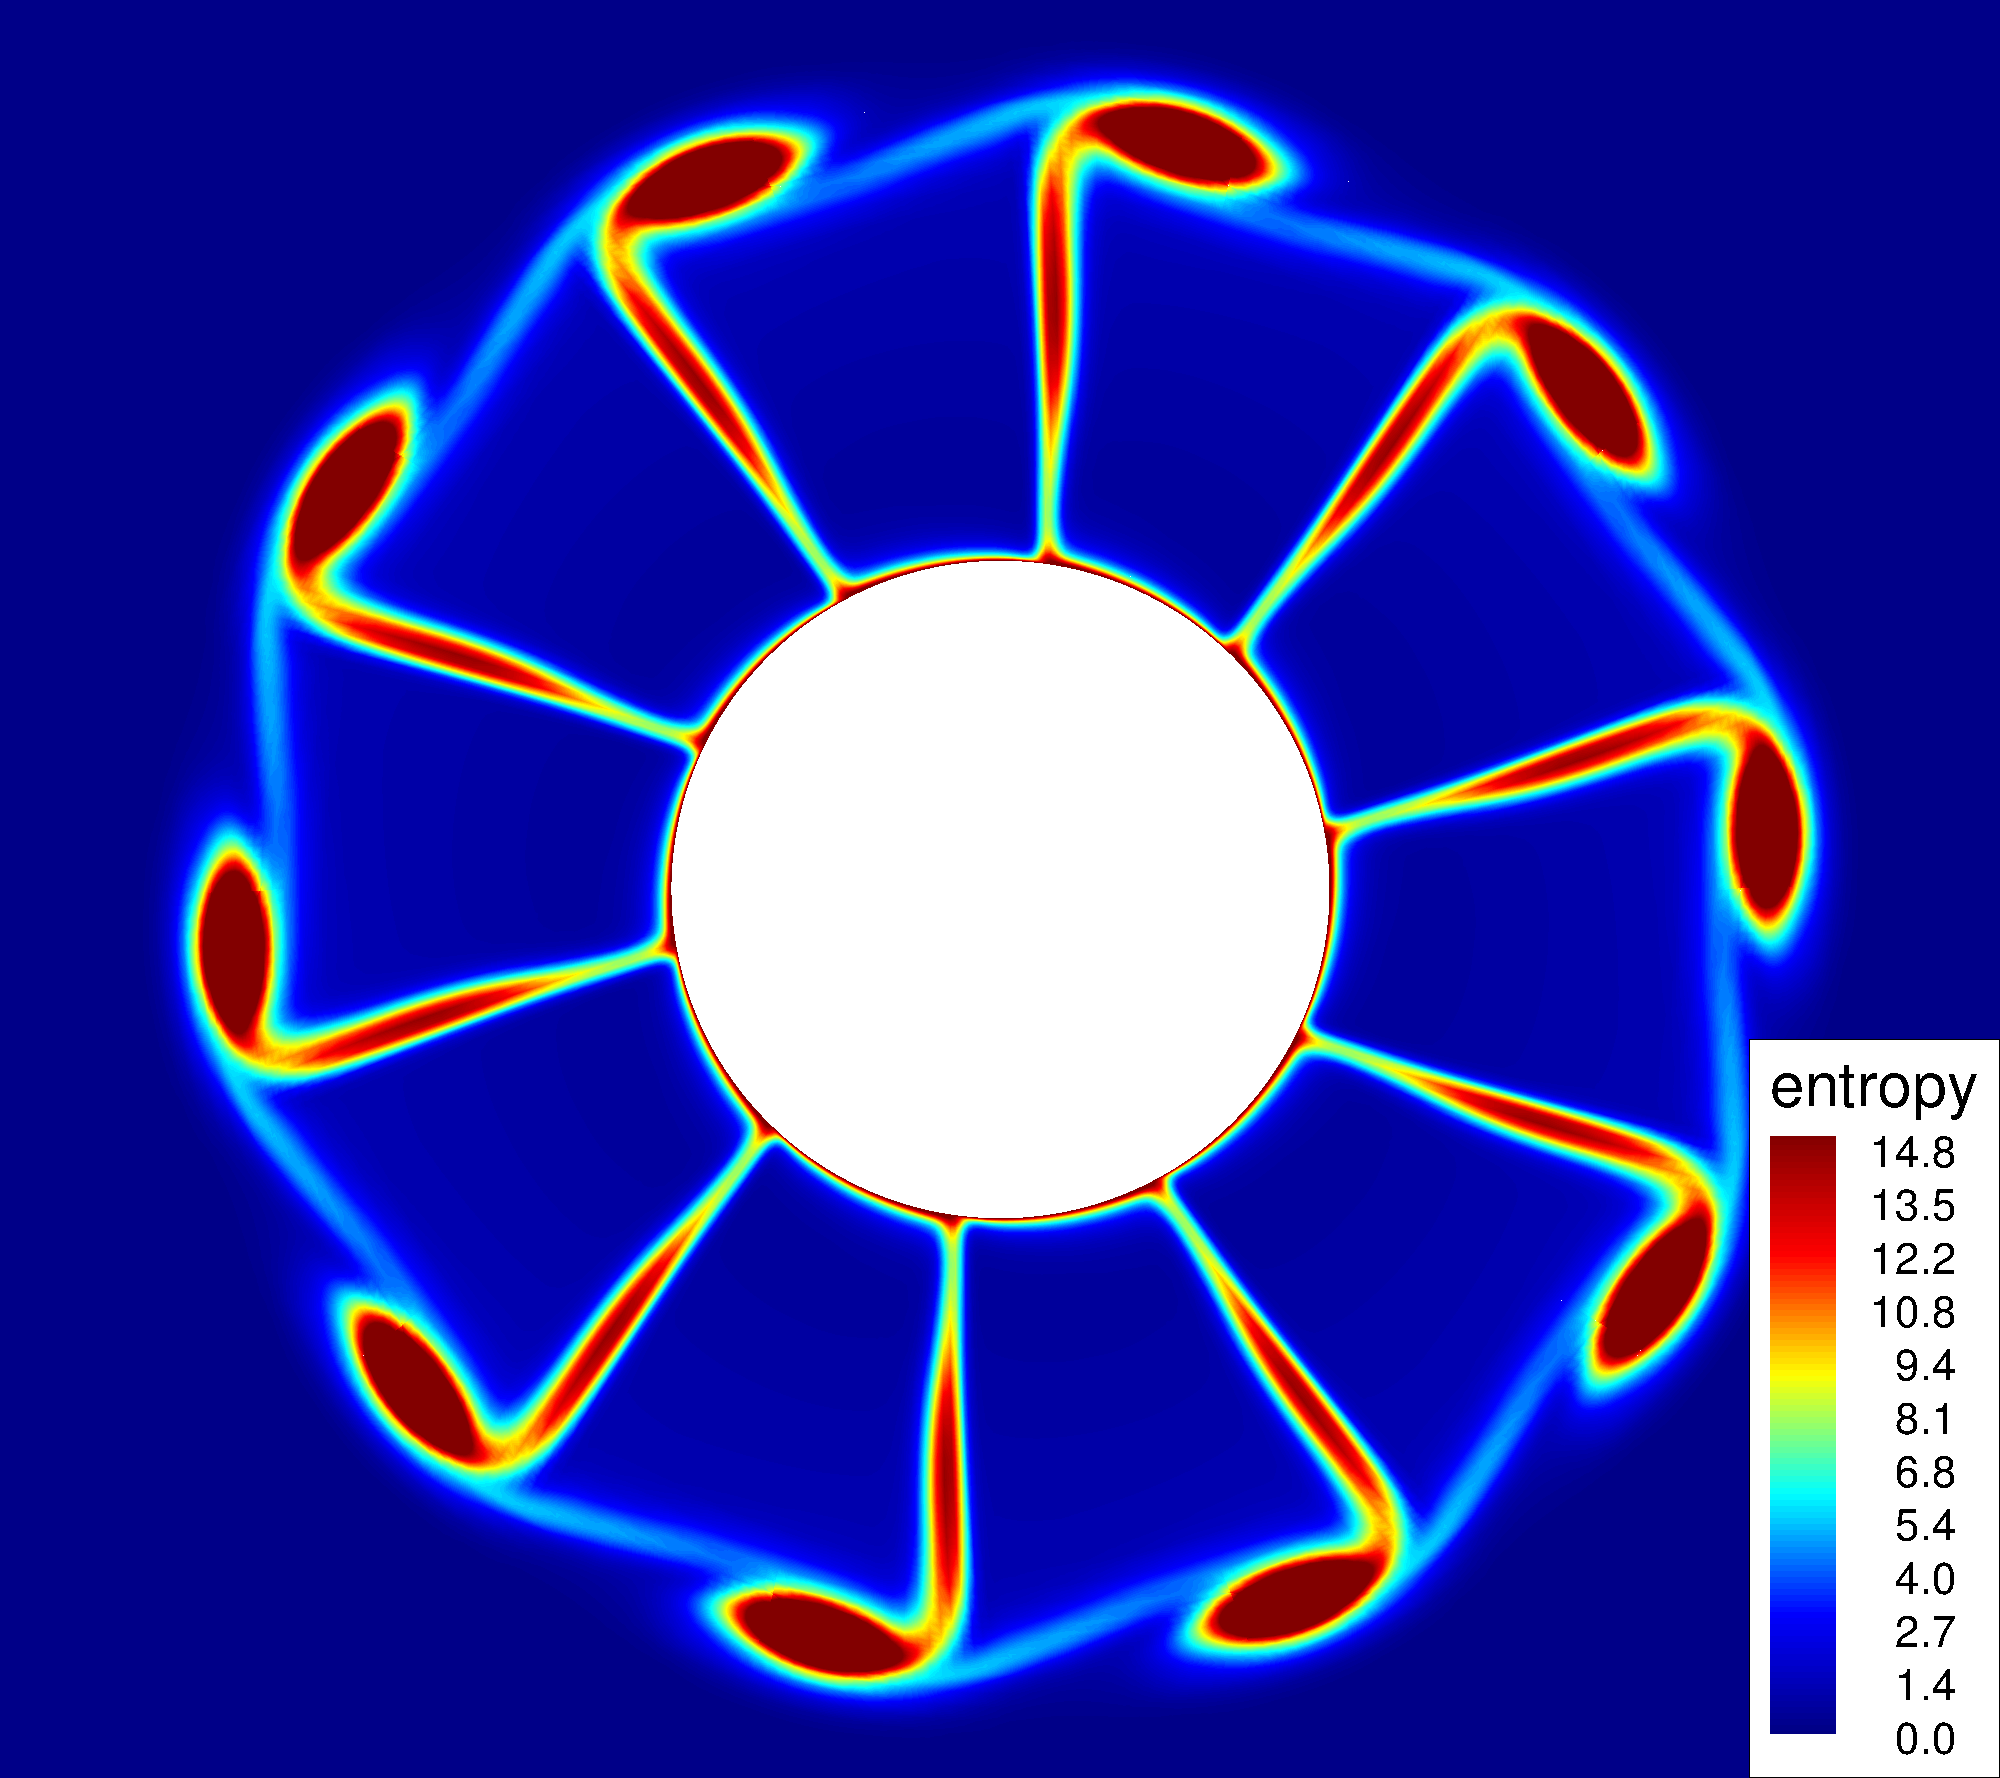
\includegraphics[width=.35\textwidth]{DREAM_LS_RANS_roe2_sa_slice_x_rear_1_entropy.png}}
  \subfigure[$P6$]{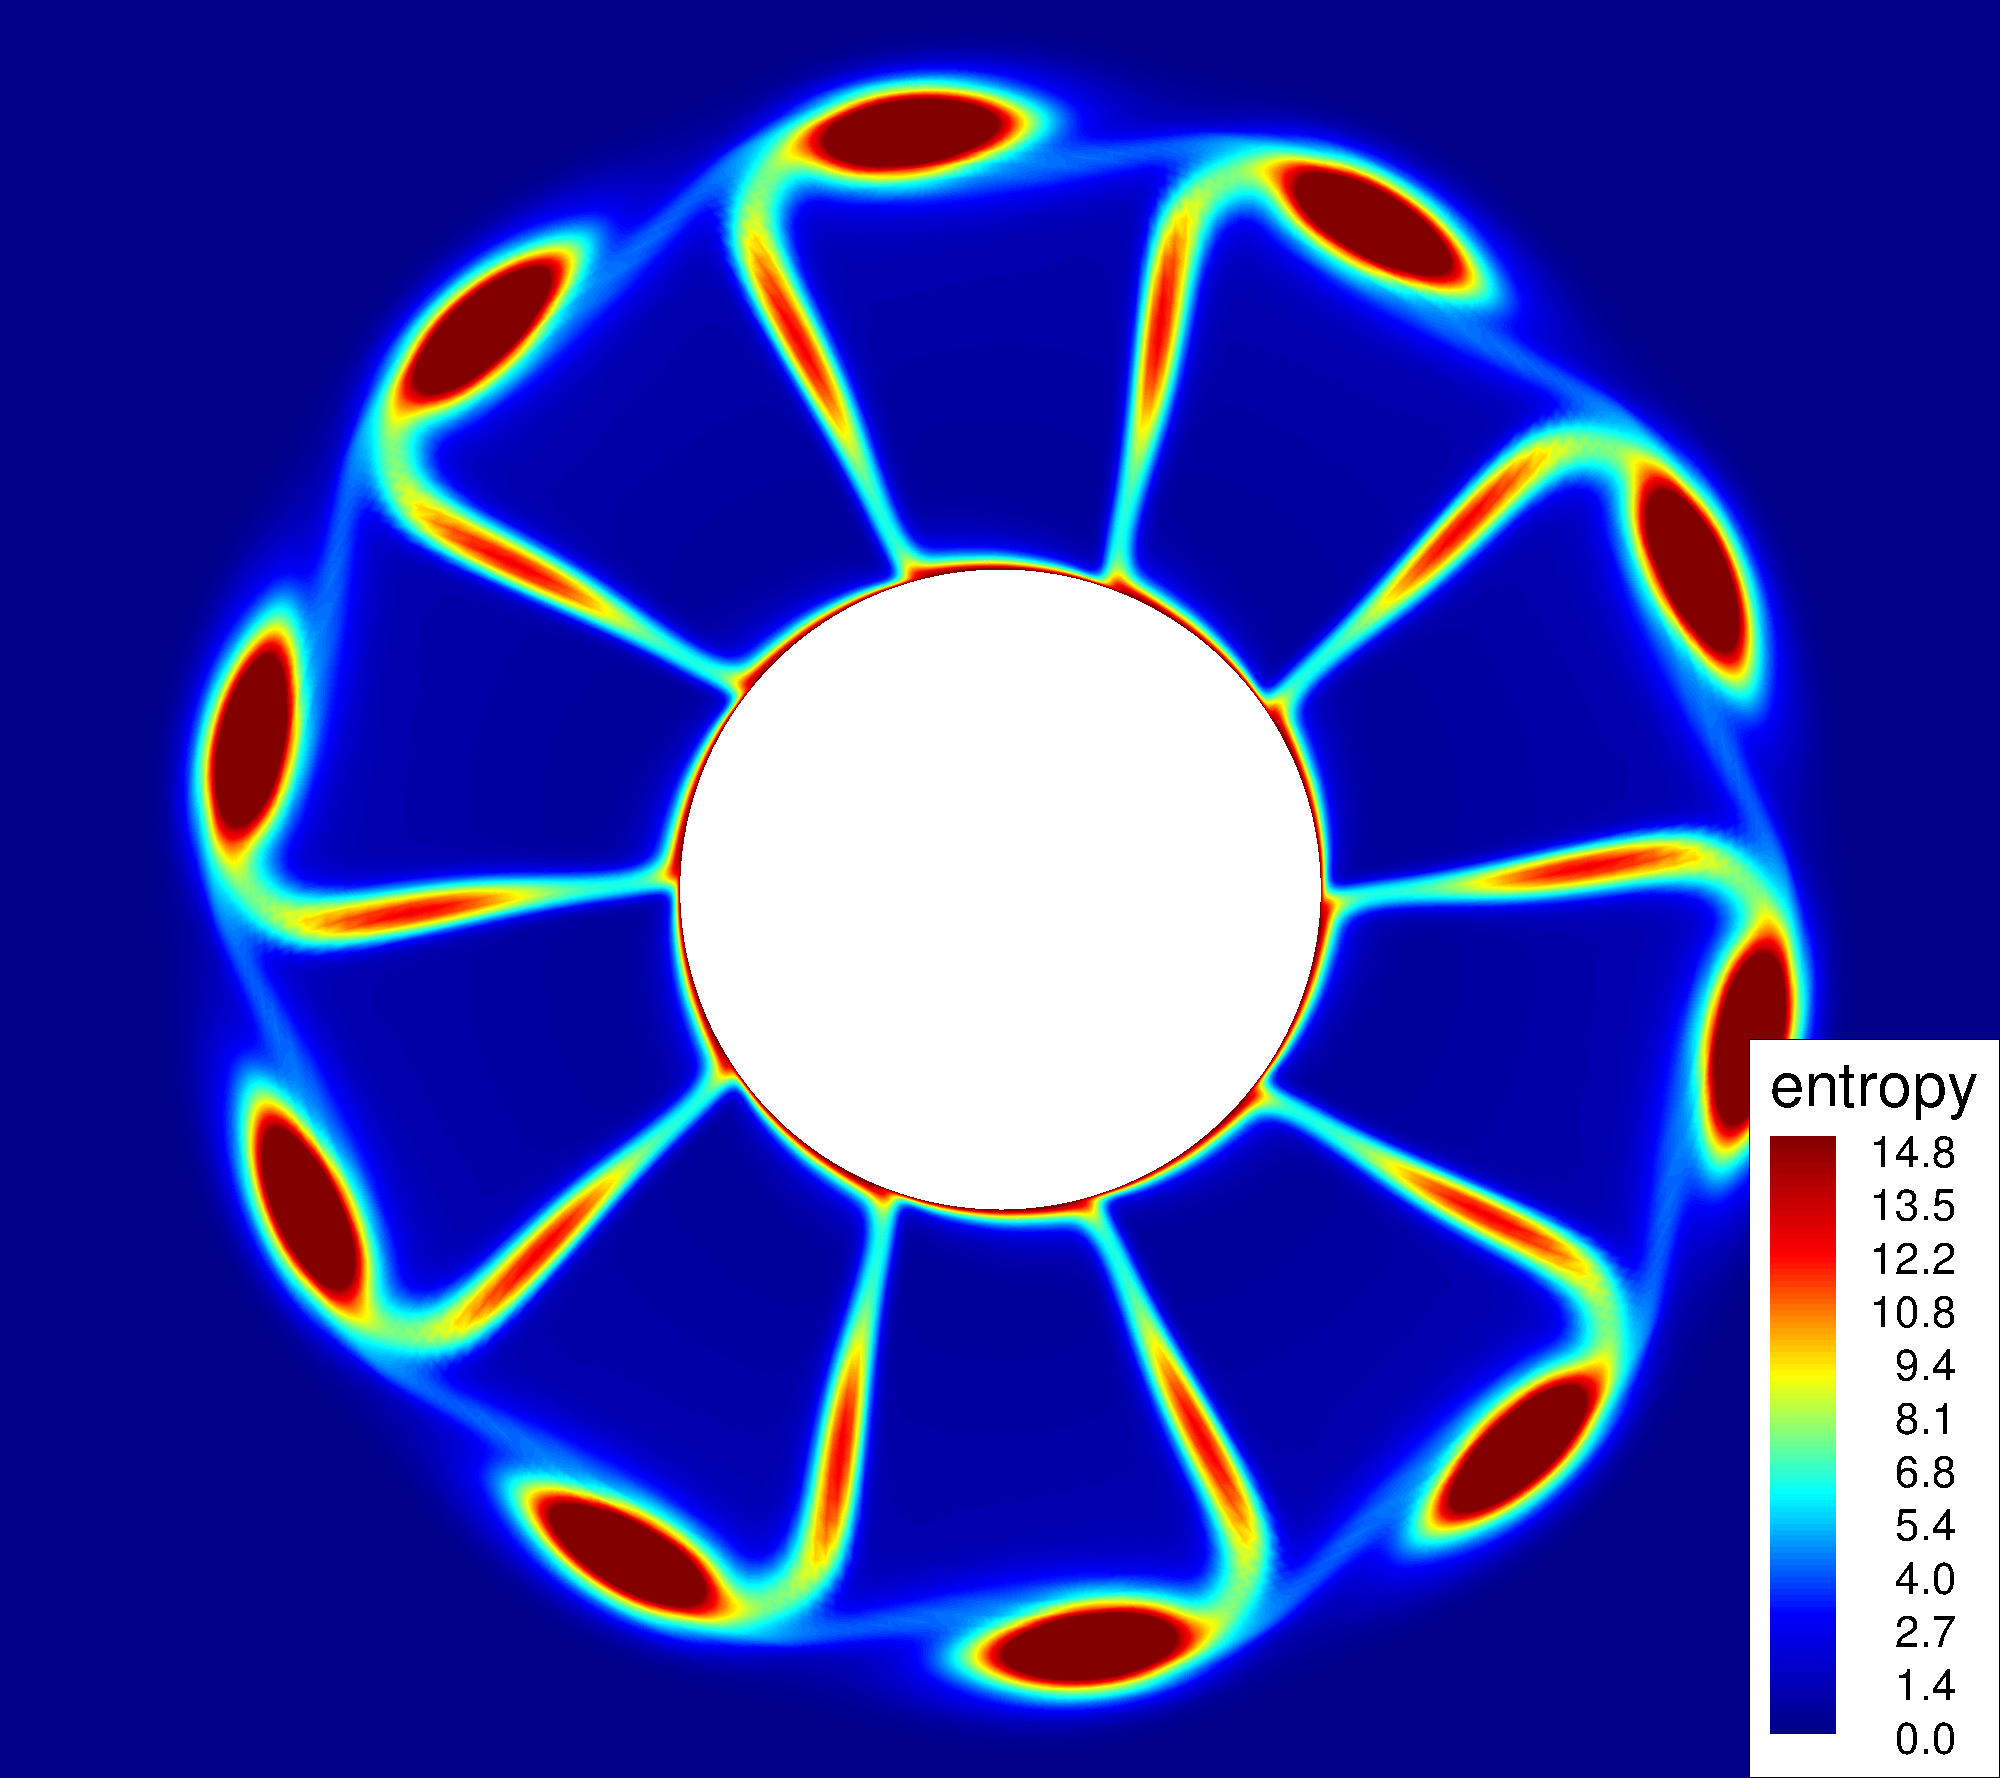
\includegraphics[width=.35\textwidth]{DREAM_LS_RANS_roe2_sa_slice_x_rear_2_entropy.png}}
  \caption{}
\end{figure}